\documentclass[11pt]{article}

\usepackage{a4wide}

 
\usepackage[T1]{fontenc} 
\usepackage[scaled=.7]{beramono}
\usepackage{lmodern}  
\usepackage[utf8]{inputenc}
%\usepackage[english]{babel}      
\usepackage{amsmath}
\usepackage{amssymb}  
\usepackage{amsfonts}
\usepackage{amsthm}
\usepackage{dsfont}
\usepackage{mathrsfs}   
\usepackage{ifdraft} 
\usepackage{array,multicol}  
\usepackage{booktabs}
\usepackage{longtable}
\usepackage{cancel}
\usepackage{float}
\usepackage{stmaryrd} 
\usepackage{colortbl} 
\usepackage{caption}
\usepackage{mathpartir} 
\usepackage{mathtools}
\usepackage[final]{listings}
\usepackage{url}
%\usepackage{bibunits}% Incompatible with biblatex, see biblatex's documentation for workarounds.
\usepackage{marvosym} % Note that this exports \Cross, incompatible with package bbding.
%                     % Circumvented by code around the \usepackage{bdding} below.
\usepackage{forest}
\usepackage{tikz,datetime}
\usetikzlibrary{decorations.pathreplacing,trees,calc,fit,positioning,chains,arrows,arrows.meta,automata,shapes,graphs,shapes.geometric,shapes.symbols,
decorations.markings,patterns,matrix,decorations.pathmorphing,mindmap,math}
%,triangle-fit,decorations.growingwave,oni-squiggly}
\usepackage{pgf}
\usepackage{pgfplots}
\usepackage{graphicx}
\usepackage{subfigure}
\usepackage{alltt}
\usepackage{mathrsfs}
\usepackage{wrapfig}
\usepackage{xcolor}
\usepackage{dsfont}
\usepackage{amsbsy}
\usepackage{savesym}
% Circumvent incompatibility between marvosym and bdding, which both define \Cross.
% See https://groups.google.com/forum/#!topic/comp.text.tex/LSETDAIaJug
\savesymbol{Cross}% Save original \Cross as \origCross.
\usepackage{bbding}
\restoresymbol{bb}{Cross}% Restore original \Cross from marvosym + rename bbding's \Cross to \bbCross.
\usepackage{relsize} 
\usepackage{wasysym}
%\usepackage{growingwave}  
\pgfdeclarelayer{background}
\pgfdeclarelayer{foreground}
\pgfsetlayers{background,main,foreground}
\usepackage{epigraph} 
%\usepackage{oni-trees}
%\usepackage{oni-tree-defaults}
%\usepackage[backend=bibtex,style=authoryear,natbib=true,maxbibnames=99]{biblatex}
%% User the bibtex backend with the authoryear citation style (which
%% resembles APA) 
\usepackage{tikz,datetime}
\usetikzlibrary{decorations.pathreplacing,trees,calc,fit,positioning,chains,arrows,arrows.meta,automata,shapes,graphs,shapes.geometric,shapes.symbols,
decorations.markings,patterns,matrix,decorations.pathmorphing,mindmap,math}
%,triangle-fit,decorations.growingwave,oni-squiggly}
\usepackage{pgf}
\usepackage{pgfplots}
\usepackage{graphicx}
\usepackage{subfigure}

%%%%%%%%%%
%% from main.tex




\newtheorem{definition}{Definition}

\newcommand{\snumber}[1]{\textrm{{\scriptsize(#1)}}}

%%%%%
%%%%% From Chapter on SSMART
\newcommand{\disp}[1]{\lstinline&#1&}

%% True label
\def\lbtrue{\textsf{true}}
%% False Label
\def\lbfalse{\textsf{false}}


%Set of structure field identifiers
\def\fset{\ensuremath{\mathcal{F}}}
%Set of variant constructors identifiers
\def\cset{\ensuremath{\mathcal{C}}}
%Set of variable identifiers
\def\vset{\ensuremath{\mathcal{V}}}
%Set of writeable variable identifiers
\def\wrvset{\ensuremath{\mathcal{V}^{+}}}
%Set of read-only variable identifiers
\def\rovset{\ensuremath{\mathcal{V}^{-}}}
%Universe of type identifiers
\def\utyp{\ensuremath{\mathbb{T}}}
%Set of base type identifiers
\def\basetyp{\ensuremath{T_0}}
%Universe of semantic values
\def\uval{\ensuremath{\mathbb{D}}}
%Typing environment
\def\tenv{\ensuremath{\Gamma}}
%Valuation
\def\env{\ensuremath{E}}

%% Types
\def\primtyp{\tau}

%Structure Type
\newcommand{\plainstype}[6]
{\ensuremath{\boldsymbol{struct}\{#1_{#2}: #3, \ldots, #4_{#5}: #6 \}}}

\newcommand{\plainmiddlestype}[9]
{\ensuremath{\boldsymbol{struct}\{#1_{#2}: #3, \ldots, #4_{#5}: #6  , \ldots,#7_{#8}: #9\}}}

\def\commonstype{\plainstype{f}{1}{\tau}{f}{n}{\tau}}
\def\commonstypeindex{\plainstype{f}{1}{\tau_1}{f}{n}{\tau_n}}
\def\commonmiddlestype{\plainmiddlestype{f}{1}{\tau_1}{f}{i}{\tau_i}{f}{n}{\tau_n}}

%Variant Type
\newcommand{\plainvtype}[6]
{\ensuremath{\boldsymbol{variant}[#1_{#2}: #3 \ver \ldots \ver #4_{#5}: #6]}}

\newcommand{\plainmiddlevtype}[9]
{\ensuremath{\boldsymbol{variant}[#1_{#2}: #3 \ver \ldots \ver #4_{#5}: #6 \ver \ldots \ver #7_{#8}: #9]}}

\def\commonvtype{\plainvtype{C}{1}{\tau}{C}{n}{\tau}}
\def\commonvtypeindex{\plainvtype{C}{1}{\tau_1}{C}{n}{\tau_n}}
\def\commonmiddlevtype{\plainmiddlevtype{C}{1}{\tau_1}{C}{i}{\tau_i}{C}{n}{\tau_n}}

%Array Type
\newcommand{\plainatype}[2]
{\ensuremath{\boldsymbol{arr}^{#1} \langle #2 \rangle}}

\def\commonatype{\plainatype{\tau}{\tau}}
\def\commonatypeindex{\plainatype{\tau_i}{\tau}}

% Values

%Structure Values
\newcommand{\plainsval}[6]
{\ensuremath{\{#1_{#2} = #3, \ldots, #4_{#5} = #6\}}}

\newcommand{\plainmiddlesval}[9]
{\ensuremath{\{#1_{#2} = #3, \ldots, #4_{#5} = #6, \ldots, #7_{#8} = #9\}}}

\def\commonsval{\plainsval{f}{1}{v_1}{f}{n}{v_n}}
\def\commonmiddlesval{\plainmiddlesval{f}{1}{v_1}{f}{i}{v_i}{f}{n}{v_n}}

%% %Variant Values
%% \newcommand{\plainvval}[4]
%% {\ensuremath{#1_{#2}[#3_{#4}] }}

%% \newcommand{\plainvvalindex}[1]
%% {\ensuremath{C_{#1}[v_{#1}]}}

%% \def\commonvval{\plainvval{C}{i}{v}{i}}

%Array Values
\def\asup{\mathcal{P}}

%% Built-in Statements
\def\unop{\ensuremath{\boldsymbol{nop}}}
\newcommand{\plainasgn}[2]{\ensuremath{#1 := #2}}
\def\commonasgn{\plainasgn{o}{e}}
\newcommand{\plaineqtest}[2]{\ensuremath{#1 = #2}}
\def\commoneqtest{\plaineqtest{e_1}{e_2}}
\newcommand{\recordnew}{r := \{e_1, \ldots, e_n \}}
\newcommand{\recordall}{\{o_1, \ldots, o_n \} := r}
\newcommand{\recordset}{r' := \{r\; \boldsymbol{with}\; f_i = e \} }
\newcommand{\recordget}{o := r.f_i}
\newcommand{\recordeq}{r' = \langle  f_1, \ldots, f_k \rangle r''}
\newcommand{\varcons}{v := C_p[e]}
\newcommand{\varswitch}
{\boldsymbol{switch}(v) \;\boldsymbol{as} \;[o_1 \arrowvert \ldots \arrowvert o_n ]}
\newcommand{\varpossible}{v \in \{ C_1,\ldots ,C_k \}}
\newcommand{\arrayget}{o := a[i]}
\newcommand{\arrayset}{a' := [a \; \boldsymbol{with} \; i = e]}

\newcommand{\predcall}
{p(e_1, \ldots, e_n) \; [\lambda_1: \bar{o}_1 \; \arrowvert \ldots \arrowvert \; \lambda_m: \bar{o}_m]}
\newcommand{\pcall}
{
{p(e_1, \ldots, e_n)\newline
[\lambda_1: \bar{o}_1 \; \arrowvert \ldots \arrowvert \; \lambda_m: \bar{o}_m]}
}

%% Exit Labels

%% True label
\def\lbtrue{\textsf{true}}
%% False Label
\def\lbfalse{\textsf{false}}

%labels-outputs maps macros  
\newcommand{\unary}[1]{\left[\begin{array}{ccc}
              \lbtrue &\mapsto &#1\\
              \end{array}
       \right]}

\newcommand{\lbinary}[2]{
  \left[\begin{array}{c}
      \lbtrue \mapsto #1\\ 
      \lbfalse \mapsto #2
    \end{array}\right]
}

\newcommand{\multi}[4]{\left[\begin{array}{ccc}
              \lambda_{#1} &\mapsto & \bar{o}_{1}\\
               \vdots   &\ddots &\vdots \\
              \lambda_{#2} &\mapsto & \bar{o}_{#4}
              \end{array}
       \right]}

\newcommand{\multiv}[3]{\left[\begin{array}{ccc}
              \lambda_{#1} &\mapsto &o_{1}\\
               \vdots   &\ddots &\vdots \\
              \lambda_{#2} &\mapsto &o_{#3}
              \end{array}
       \right]}




%%%%%
%%%%% From Chapter on SMIL
\def\asmil{\textsf{$\alpha$Smil}}

\def\commonvval{\plainvval{C}{i}{v}}

%Generic option type
\def\optiont{\boldsymbol{\small{variant}}
[\textrm{\disp{Some}} : \boldsymbol{\small{struct}}\{\textrm{\disp{t}} : \textrm{\disp{T}}\} \; 
\arrowvert\; 
\; \textrm{\disp{None}} : \boldsymbol{\small{struct}}\{\}]}

%%%%% Chapter 5
\def\ileq{\dleq_{\intra}}
%\def\ijoin{\vee_{\intra}}
\def\ireduce{\oplus_{\intra}}
\def\uintra{\mathscr{D}}


%% misc macros
\newcommand{\ver}{\arrowvert \;}

%macros tables (chapters 5 and 7)
%!%!%! Does this impact tables in other chapters?
%!%!%!     If so, we can put it in a \begingroup \endgroup, so that it affects only the desired tables
\newcommand{\ra}[1]{\renewcommand{\arraystretch}{#1}} 
\colorlet{tableheadcolor}{gray!25} % Table header colour = 25% gray
\newcommand{\headcol}{\rowcolor{tableheadcolor}} %
\colorlet{tablerowcolor}{gray!10} % Table row separator colour = 10% gray
\newcommand{\rowcol}{\rowcolor{tablerowcolor}} %
\colorlet{tablerowcolor}{gray!10} % Table row separator colour = 10% gray %!%!%! was not in chapter 5.

% math operators with subscript-ish
%Macro big meet
\makeatletter
\newlength{\widthofMeet}
\newlength{\widthofR}

\newsavebox{\boxname}
\newsavebox{\boxnameb}
\newsavebox{\boxnamec}

\def\negphantomdiff#1#2#3{%
  \def\resetstyle{#1}
  \savebox{\boxname}{$#1#2$}%
  \savebox{\boxnameb}{$#1#3$}%
  \hspace{-\wd\boxnameb}\hspace{\wd\boxname}% negative width of just the R (= - whole + wedge)
}
\def\withwidthoffirst#1#2#3{%
  \def\resetstyle{#1}
  \savebox{\boxname}{$#1#2$}%
  \savebox{\boxnameb}{$#1#3$}%
  \hspace{\wd\boxnameb}\hspace{-\wd\boxname}%width of just the R (= whole - wedge)
  \usebox{\boxnameb}%
}
\def\alignedmathop#1#2{%
  \@ifstar{%
    \centeredmathop{#1}{#2}%
  }{%
    \mathchoice%
    {\negphantomdiff{\displaystyle}{#1}{#2}}% <--- HERE displaystyle
    {\negphantomdiff{\textstyle}{#1}{#2}}% <--- HERE textstyle
    {\negphantomdiff{\scriptstyle}{#1}{#2}}% <--- HERE scriptstyle
    {\negphantomdiff{\scriptscriptstyle}{#1}{#2}}% <--- HERE scriptscriptstyle
    \centeredmathop{#1}{#2}%
  }%
}
\def\centeredmathop#1#2{%
  \mathop{%
    \mathchoice%
    {\withwidthoffirst{\displaystyle}{#1}{#2}}% <--- HERE displaystyle
    {\withwidthoffirst{\textstyle}{#1}{#2}}% <--- HERE textstyle
    {\withwidthoffirst{\scriptstyle}{#1}{#2}}% <--- HERE scriptstyle
    {\withwidthoffirst{\scriptscriptstyle}{#1}{#2}}% <--- HERE scriptscriptstyle
  }%
}
\makeatother

% Needed to appear cleanly in the list of symbols
\def\intrachapfive{\Delta}
\def\ijoinchapfive{%
  \alignedmathop{%
    \vee%
  }{%
    \mathchoice%
    {\vee\mkern-4mu\smash{\raisebox{-0.3ex}{$\resetstyle\mathlarger{{}_{\intrachapfive}}$}}}%
    {\vee\mkern-3mu\smash{\raisebox{-0.1ex}{$\resetstyle\mathlarger{{}_{\intrachapfive}}$}}}%
    {\vee\mkern-2.25mu\smash{\raisebox{-0.3ex}{$\resetstyle\mathlarger{{}_{\intrachapfive}}$}}}%
    {\vee\mkern-2.5mu\smash{\raisebox{-0.35ex}{$\resetstyle\mathlarger{{}_{\intrachapfive}}$}}}%
  }%
}





\title{Static analysis for proof obligation elimination in functional
  specifications}

\author{Oana Andreescu \and Thomas Jensen \and St\'ephane Lescuyer}

\date{\today}

\begin{document}

\begin{abstract}

\end{abstract}


\section{Introduction}

\subsection{The frame problem}

The frame problem~\cite{mccarthy69} was identified and described at
least as early as 1969 by McCarthy and Hayes, in the context of
Artificial Intelligence (AI). The initial description of the
frame problem is the following:

\begin{quotation}
``In proving that one person could get into conversation with another, we were
  obliged to add the hypothesis that if a person has a telephone he still has it
  after looking up a number in the telephone book. If we had a number of actions
  to be performed in sequence we would have quite a number of conditions to
  write down that certain actions do not change the values of certain
  fluents. In fact, with $n$ actions and $m$ fluents we might have to write down
  $mn$ such conditions.''
\end{quotation}

Unsurprisingly, 
%given its identification in the context of logicist AI, 
the frame problem manifests itself in the realm of formal software
specification and deductive verification as well~\cite{borgida93}.
Deductive verification methods consist in producing formal correctness
proofs, by first generating a set of formal mathematical proof
obligations from the program and its specification, and by
subsequently discharging these. Proof
obligations can sometimes be discharged automatically by using static
analysis and decision procedures, but  often they require the use of
an interactive prover. Reducing the number of proof obligations in a
verification hence becomes an essential task. 

A large part of a proof consists in proving that a global invariant is
preserved, despite the state changes that a program makes
as it executes.  A number of proof obligations deal with those parts of the
state that actually have been changed. Another set of proof
obligations arise from dealing with the part of the state that does
not change. These may be particularly tedious to handle because it 
should be ``evident'' that the invariant holds for this part of the
state. As a consequence, several specification formalisms offer the
possibility of specifying what is changed and what does not
change. These properties are called \emph{frame properties}.

Frame properties help reducing the number of proof
obligations. However, specifying frame properties might not seem dramatic
on small examples, but in real-world examples this quickly
escalates, leading to the necessity of specifying a plethora of
conditions.Writing such conditions is necessary but also notoriously
repetitive and tedious.  As Kogtenkov et al.~\cite{kogtenkov15}
so eloquently puts it:

\begin{quotation}
``It is hard enough to convince  programmers to state what their program does; forcing 
them in addition to specify all that it does not do may be a tough sell.'' 
\end{quotation}

The tedious, undeserved, manual effort entailed by the specification and
verification of frame properties is a manifestation of the frame problem. Though
certain conventions and approaches, such as the \emph{implicit frames} approach,
for specifying frame properties can alleviate the manual effort imposed, some
manifestation of the frame problem will be visible to some extent in the context
of any specification language and verification method.

The article proposes a solution to the frame problem based on
fully-automatic, static program analyses for inferring the
preservation of program invariants. More specifically, we target the
automatic identification of properties that depend only on an input
subset that is disjoint from an operation's \emph{frame}, i.e. the
state subset it modifies.

\subsection{Methodology}

To this end, we propose a solution based on static analysis which does not
require any additional frame annotations. By detecting the subset
on which a property depends and by uncovering the part that is not modified by
an operation, as shown in Figure~\ref{ch1:fig:strategy}, we can automatically
discharge proof obligations related to unmodified parts. We employ two different
static analyses for this goal.

\begin{figure}[!h]
%Second Line
\begin{minipage}[c]{0.1\textwidth}
\[
\begin{array}[b]{crcl} 

\textrm{{Dependency}} & 
Obs
\left(
\mathord{%
\resizebox{\textwidth}{!}{
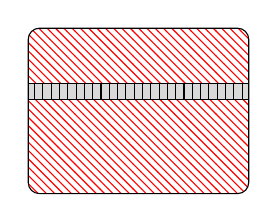
\begin{tikzpicture}[ baseline= (current bounding box.center), scale=0.7, auto] 
    \filldraw[fill=lightgray!60,pattern = north west lines, pattern color=red, rounded corners]  (4.5,-8.5) rectangle (8.5,-5.5); 
    \filldraw[fill=lightgray!60] (4.5, -6.5) rectangle (8.5, -6.8); 
    \filldraw[fill=lightgray!60,pattern=vertical lines, pattern color=black] (4.5, -6.5) rectangle (8.5, -6.8); 
\end{tikzpicture}%
}
}
\right)
 & = &
Obs
\left(
\mathord{%
\resizebox{\textwidth}{!}{

\begin{tikzpicture}[baseline=(current bounding box.center), scale=0.7, auto]
  \filldraw[fill=red!75!black, rounded corners] (12,-12) rectangle (16,-9) ;% draw/fill the box
  \filldraw[pattern = north east lines, pattern color=white, rounded corners]  (12,-12) rectangle (16,-9) ;% draw the stripes
  \filldraw[fill=lightgray!40] (12, -10) rectangle (16, -10.3);
  \filldraw[pattern=vertical lines, pattern color=black] (12, -10) rectangle (16, -10.3);
\end{tikzpicture}%
}
}
\right) \\[1.5em]
 
\textrm{{Correlation}} &
\textrm{\huge{$f$}}
\left (
\mathord{%
\resizebox{\textwidth}{!}{ 

\begin{tikzpicture}[baseline=(current bounding box.center), scale=0.7, auto]
    \filldraw[fill=lightgray!60, rounded corners]  (1,-10) rectangle (5,-7) 
    node[scale=1.5,rectangle, minimum size = 2] at (3,-7.5) {\Large$?$} 
    node[scale=1.5,rectangle, minimum size = 2] at (3, -9) {\Large$?$}; 
    \filldraw[fill=lightgray!60] (1, -8) rectangle (5, -8.3); 
    \filldraw[fill=lightgray!60,pattern=vertical lines, pattern color=black] (1, -8) rectangle (5, -8.3); 
\end{tikzpicture}%
}
}
\right)
&  =  &
\mathord{%
\resizebox{\textwidth}{!}{
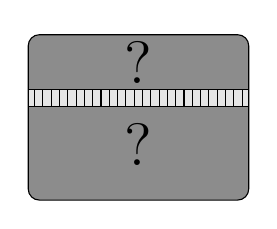
\begin{tikzpicture}[baseline=(current bounding box.center), scale=0.7, auto]
        \filldraw[fill=darkgray!60, rounded corners]  (12,-10) rectangle (16,-7) 
            node[scale=1.5,rectangle, minimum size = 2] at (14,-7.5) {\Large$?$}
            node[scale=1.5,rectangle, minimum size = 2] at (14, -9) {\Large$?$};;% draw the box
       \filldraw[fill=lightgray!40] (12, -8) rectangle (16, -8.3);
    \filldraw[fill=lightgray!40,pattern=vertical lines, pattern color=black] (12, -8) rectangle (16, -8.3);
\end{tikzpicture}%
}
} \\[1.5em]

\textrm{{Invariant}} &
Obs
\left (
\mathord{%
\resizebox{\textwidth}{!}{
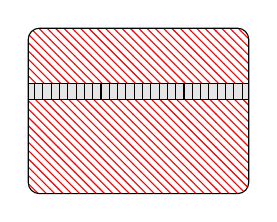
\begin{tikzpicture}[baseline=(current bounding box.center), scale=0.7, auto]
    \filldraw[fill=lightgray!40,pattern = north west lines, pattern color=red, rounded corners]  (1,-12) rectangle (5,-9); 
    \filldraw[fill=lightgray!40] (1, -10) rectangle (5, -10.3); 
    \filldraw[fill=lightgray!40,pattern=vertical lines, pattern color=black] (1, -10) rectangle (5, -10.3); 
\end{tikzpicture}%
}
}
\right)
 & \Rightarrow & Obs
\left (
\textrm{\huge{$f$}}
\left(
\mathord{%
\resizebox{\textwidth}{!}{
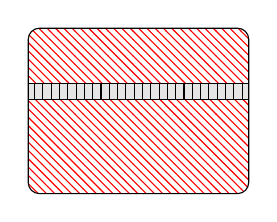
\begin{tikzpicture}[baseline=(current bounding box.center), scale=0.7, auto]
        \filldraw[fill=lightgray!40,pattern = north west lines, pattern color=red, rounded corners]  (12,-12) rectangle (16,-9) ;% draw the box
       \filldraw[fill=lightgray!40] (12, -10) rectangle (16, -10.3);
    \filldraw[fill=lightgray!40,pattern=vertical lines, pattern color=black] (12, -10) rectangle (16, -10.3);
\end{tikzpicture}%
}
}
\right)
\right) 
\end{array}
\]
\end{minipage}
\caption{Frame Problem and Solution Strategy}
\label{ch1:fig:strategy}
\end{figure}

The first analysis of our two-step strategy is a \emph{dependency
  analysis}, which detects the input subset $\delta$ on which the
outcome of an operation or of a logical property $\mathscr{L}$
relies. This subset is represented by the grey rectangle with vertical
lines in Figure~\ref{ch1:fig:frameproblem}. The second is a
\emph{correlation analysis}, meant to detect the subset $\xi$ modified
by an operation $\mathscr{O}$, illustrated by the orange
rectangles with inclined lines in
Figure~\ref{fig:frameproblem}. By employing these two static
analyses, thus detecting $\delta$ and $\xi$ automatically, and by
subsequently reasoning based on their combined results, we can infer
the preservation of the property $\mathscr{L}$ for the post-state of
$\mathscr{O}$.

\subsection{Application context: Formal verification of systems software}

\subsection{Organisation of the article}

\section{The SMART functional specification language}

\section{Dependency analysis}

%%% Macros %%%

%% % Values

%% %Variant Values
%% \newcommand{\plainvval}[4]
%% {\ensuremath{#1_{#2}[#3_{#4}] }}

%% \newcommand{\plainvvalindex}[1]
%% {\ensuremath{C_{#1}[v_{#1}]}}

%% \def\commonvval{\plainvval{C}{i}{v}{i}}


%% Dependency macros

%% \addto\captionsenglish{
%% \renewcommand{\tablename}{Figure}
%% }
\newcolumntype{L}[1]{>{\raggedright}m{#1}}
%misc macros
\newcommand{\comment}[1]{\ifdraft{\small\textbf{#1}}{}}

\def\inputs{\ensuremath{\mathcal{I}}}
\def\writ{\mathscr{V}^{+}}

\newcommand\mmyrbox[2][fill=red!20]{%
    \tikz[baseline]\node[%
        inner ysep=0pt, 
        inner xsep=2pt, 
        anchor=text, 
        rectangle, 
        rounded corners=1mm,
        #1] {\strut#2};%
}

\newcommand\mmygbox[2][fill=lightgray!30]{%
    \tikz[baseline]\node[%
        inner ysep=0pt, 
        inner xsep=2pt, 
        anchor=text, 
        rectangle, 
        rounded corners=1mm,
        #1] {\strut#2};%
}

\def\everything{\ensuremath \top}
\def\nothing{\ensuremath \oslash}
\def\impossible{\ensuremath \bot}

%dependency domain macros
\def\udep{\mathcal{D}}
\def\dom{\mathit{\delta}}
\newcommand{\structdom}[2]{\{#1; \ldots; #2\}}
\newcommand{\vardom}[2]{[#1; \ldots; #2]}
\newcommand{\adom}[1]{\langle #1 \rangle} 
\newcommand{\aexcdom}[3]{\langle #1 \triangleright #2: \; #3 \rangle}
\newcommand{\adomusual}{\langle \dom_{\mathit{def}} \triangleright i \;: \; \dom_{\mathit{exc}} \rangle}
\newcommand{\addef}{\langle \dom_{\mathit{def}} \triangleright i \;: \; \dom_{\mathit{exc}} \rangle}

\newcommand{\dstruct}[1]{f_{#1} \mapsto \dom_{#1}}
\newcommand{\dostruct}[1]{f_{#1} \mapsto \dom'_{#1}}
\newcommand{\djstruct}[1]{f_{#1} \mapsto \dom_{#1} \vee \dom'_{#1}}
\newcommand{\djnothingstruct}[1]{f_{#1} \mapsto \oslash \vee \dom_{#1}}
\newcommand{\dmstruct}[1]{f_{#1} \mapsto \dom_{#1} \oplus \dom'_{#1}}


\newcommand{\dvar}[1]{C_{#1} \mapsto \dom_{#1}}
\newcommand{\dovar}[1]{C_{#1} \mapsto \dom'_{#1}}
\newcommand{\djvar}[1]{C_{#1} \mapsto \dom_{#1} \vee \dom'_{#1}}
\newcommand{\djnothingvar}[1]{C_{#1} \mapsto \oslash \vee \dom_{#1}}
\newcommand{\dmvar}[1]{C_{#1} \mapsto \dom_{#1} \oplus \dom'_{#1}}

\newcommand{\deferred}[1]{\textrm{\textbf{\textsf{Deferred}}}(#1)}


\newcommand{\subst}{\blacktriangleleft(\sigma, \phi)}

\def\ddef {\ensuremath{\mathit{\dom_{def}}}}
\def\dexc {\ensuremath{\mathit{\dom_{exc}}}}
\def\dodef{\ensuremath{\mathit{\dom'_{def}}}}
\def\doexc{\ensuremath{\mathit{\dom'_{exc}}}}

\def\dleq{\sqsubseteq}

%intra macros
\def\intra{\Delta}

%inter macro
\def\inter{\mathscr{D}}
%% \def\defstruct{ \{.f_1\pi_1, \; \ldots, \; .f_n\pi_n\} }
%% \def\defstructo{ \{.f_1\pi'_1, \; \ldots, \; .f_n\pi'_n\} }
%% \def\defvar{[@C_1\pi_1, \; \ldots, \;@C_n\pi_n]}
%% \def\defvaro{[@C_1\pi'_1, \; \ldots, \;@C_n\pi'_n]}
%% \def\defcell{\langle i \rangle \pi_{\mathit{exc}}}
%% \def\defcello{\langle i \rangle \pi'_{\mathit{exc}}}
%% \def\defout{\langle * \setminus i \rangle \pi_{\mathit{out}}}
%% \def\defouto{\langle * \setminus i \rangle \pi'_{\mathit{out}}}
%% \def\defarr{\langle * \rangle \pi_{\mathit{def}}}
%% \def\defarro{\langle * \rangle \pi'_{\mathit{def}}}
%% \def\pexc{\pi_{\mathit{exc}}}
%% \def\pdef{\pi_{\mathit{def}}}
%% \def\piout{\pi_{\mathit{out}}}
%% \def\pleq{\underset{\circ}{\dleq}}
%% \def\pjoin{\underset{\circ}{\vee}}
%% \def\pf{\underset{\circ}{.f}}
%% \def\pc{\underset{\circ}{@C}}
%% \def\pind{\underset{\circ}{\langle i \rangle}}
%% \def\pout{\underset{\circ}{\langle * \setminus i \rangle}}
%% \def\parr{\underset{\circ}{\langle * \rangle}}
%% \def\wtpath{\underset{\circ}{\vdash}}
%% \def\wfpath{\underset{\circ}{\vDash}}
%% \def\app{\mathit{::}\pi_a }
%% \def\appf{\mathit{::}.f }
%% \def\appc{\mathit{::}@C }
%% \def\appa{\mathit{::}\langle * \rangle}
%% \def\appo{\mathit{::}\langle * \setminus i \rangle}
%% \def\appi{\mathit{::}\langle i \rangle}

%equations macros
\newcommand{\transfer}[3]{\llbracket#2\rrbracket_{#3}(#1)}
\newcommand{\killo}[2]{(\intra_{#1} \setminus #2)}
\def\binlabels{
 \begin{tabular}{@{}l@{}}
$\lambda_{true}$ \\\\
$\lambda_{false}$ \\
\end{tabular} }
\def\ltrue{\lambda_{true}}

%join comment macros
\def\veps{\varepsilon}
\def\vepsi{\varepsilon_i}
\def\eei{(\varepsilon \vee \varepsilon_i)}
\def\ddj{(\delta \vee \delta_j)}

%projection macros
\newcommand{\projcell}[1][i]{\langle#1\rangle}
\newcommand{\projext}[1][i]{\langle * \setminus#1\rangle}
\def\projarr{\langle * \rangle}

%paths macros
%% \def\arrpath{\langle * \rangle}
%% \def\cellpath{\langle i \rangle}
%% \def\outpath{\langle * \setminus i \rangle}

%wf
\def\inps{\mathcal{I}}
\def\outs{\mathcal{O}}

% tabular column
\newcolumntype{L}[1]{>{\raggedright\let\newline\\\arraybackslash\hspace{0pt}}m{#1}}


% tikz figures for example
% Preparation for Variant, Structure and Array diagrams with arrows and red and green

\def\tmul{*1mm}
\def\dtriangle#1#2#3#4#5{%
  \tikz[remember picture, baseline={(dottriangle-x#1.base)}]{%
    \node[inner sep=0pt] (dottriangle-x#1) {\phantom{$x$}};%
    \node[dot,#2] (dottriangle-dot#1) at ($(dottriangle-x#1.base)!.5!(dottriangle-x#1.north)$) {};%
    %% The anchors and size of the isosceles triangle are not well positionned.
    % \node[draw, shape=isosceles triangle, shape border rotate=90, anchor=north,#2,isosceles triangle stretches,inner sep=0pt,minimum width=#3\tmul,minimum height=#4\tmul] (t) at (dot.center) {};
    \draw[#2] (dottriangle-dot#1.center) -- ++(.5*#3\tmul,-#4\tmul) coordinate (dottriangle-te#1) -- ++(-#3\tmul,0) coordinate (dottriangle-tw#1) -- cycle;
    \coordinate (dottriangle-tc#1) at (barycentric cs:dottriangle-dot#1=1,dottriangle-te#1=1,dottriangle-tw#1=1);
    \begin{pgfonlayer}{background}
    \node[fit=(dottriangle-dot#1) (dottriangle-te#1) (dottriangle-tw#1),#5] (dottriangle-bg#1) {};
    \end{pgfonlayer}
  }%
}

\def\defaultinnersep{1.3mm}
\tikzset{
  resetinnersep/.style={inner sep=\defaultinnersep,},
}

\def\dottriangle#1#2#3#4#5#6{%
  \node[resetinnersep,inner sep=0pt,anchor=base west,opacity=0] (predottriangle-x-#2) at #1 {\phantom{$x$}};%
  \node[resetinnersep,dot,anchor=south,#3,xshift=.5*#4\tmul,opacity=0] (predottriangle-dot-#2) at (predottriangle-x-#2.base west) {};%
  %% The anchors and size of the isosceles triangle are not well positionned.
  % \node[draw, shape=isosceles triangle, shape border rotate=90, anchor=north,#3,isosceles triangle stretches,inner sep=0pt,minimum width=#4\tmul,minimum height=#5\tmul] (t) at (dot.center) {};
  \draw[resetinnersep,#3,opacity=0] (predottriangle-dot-#2.center) -- ++(.5*#4\tmul,-#5\tmul) coordinate (predottriangle-te-#2) -- ++(-#4\tmul,0) coordinate (predottriangle-tw-#2) -- cycle;
%%%%%%%%%%%%
  % \begin{pgfonlayer}{background}
    \node[resetinnersep,fit=(predottriangle-dot-#2) (predottriangle-te-#2) (predottriangle-tw-#2)] (dottriangle-isep-#2) {};
    \node[inner sep=.7mm,fit=(predottriangle-dot-#2) (predottriangle-te-#2) (predottriangle-tw-#2),#6] (dottriangle-bg-#2) {};
  % \end{pgfonlayer}
%%%%%%%%%%%% same as above, but put above the background.
  \node[resetinnersep,inner sep=0pt,anchor=base west] (dottriangle-x-#2) at #1 {\phantom{$x$}};%
  \node[resetinnersep,dot,anchor=south,#3,xshift=.5*#4\tmul] (dottriangle-dot-#2) at (dottriangle-x-#2.base west) {};%
  %% The anchors and size of the isosceles triangle are not well positionned.
  % \node[draw, shape=isosceles triangle, shape border rotate=90, anchor=north,#3,isosceles triangle stretches,inner sep=0pt,minimum width=#4\tmul,minimum height=#5\tmul] (t) at (dot.center) {};
  \draw[resetinnersep,#3] (dottriangle-dot-#2.center) -- ++(.5*#4\tmul,-#5\tmul) coordinate (dottriangle-te-#2) -- ++(-#4\tmul,0) coordinate (dottriangle-tw-#2) -- cycle;
%%%%%%%%%%%%
  \coordinate (dottriangle-tc-#2) at (barycentric cs:dottriangle-dot-#2=1,dottriangle-te-#2=1,dottriangle-tw-#2=1);
  \node[inner sep=0pt,fit=(predottriangle-dot-#2) (predottriangle-te-#2) (predottriangle-tw-#2)] (dottriangle-boundingbox-#2) {};
}

%Some colors
\definecolor{coolgrey}{rgb}{0.55, 0.57, 0.67}
\definecolor{fgred}{rgb}{0.66, 0.13, 0.24}
\definecolor{yonder}{rgb}{0.64, 0.68, 0.82}
\definecolor{tangerine}{rgb}{1.0, 0.6, 0.4}
\definecolor{salmon}{rgb}{1.0, 0.63, 0.48}
\definecolor{caribbeangreen}{rgb}{0.0, 0.8, 0.6}
\definecolor{cream}{rgb}{1.0, 0.99, 0.82}
\definecolor{deepchampagne}{rgb}{0.98, 0.84, 0.65}
\definecolor{burntsienna}{rgb}{0.91, 0.45, 0.32}


% This is the definition of join_k
\def\bigijoin{%
  \alignedmathop{%
    \bigvee%
  }{%
    \mathchoice%
    {\bigvee\mkern-8mu\smash{\raisebox{-0.9ex}{$\resetstyle\mathlarger{\mathlarger{{}_{\intra}}}$}}}%
    {\bigvee\mkern-7mu\smash{\raisebox{-0.6ex}{$\resetstyle\mathlarger{\mathlarger{{}_{\intra}}}$}}}%
    {\bigvee\mkern-2.25mu\smash{\raisebox{-0.3ex}{$\resetstyle\mathlarger{\mathlarger{{}_{\intra}}}$}}}%
    {\bigvee\mkern-2.5mu\smash{\raisebox{-0.35ex}{$\resetstyle\mathlarger{{}_{\intra}}$}}}%
  }%
}
\def\largeijoin{%
  \alignedmathop{%
    \bigvee%
  }{%
    \mathchoice%
    {\bigvee\mkern-8mu\smash{\raisebox{-0.6ex}{$\resetstyle\mathlarger{{}_{\intra}}$}}}%
    {\bigvee\mkern-5mu\smash{\raisebox{-0.6ex}{$\resetstyle\mathlarger{\mathlarger{{}_{\intra}}}$}}}%
    {\bigvee\mkern-2.25mu\smash{\raisebox{-0.3ex}{$\resetstyle\mathlarger{\mathlarger{{}_{\intra}}}$}}}%
    {\bigvee\mkern-2.5mu\smash{\raisebox{-0.35ex}{$\resetstyle\mathlarger{{}_{\intra}}$}}}%
  }%
}
\def\ijoin{%
  \alignedmathop{%
    \vee%
  }{%
    \mathchoice%
    {\vee\mkern-4mu\smash{\raisebox{-0.3ex}{$\resetstyle\mathlarger{{}_{\intra}}$}}}%
    {\vee\mkern-3mu\smash{\raisebox{-0.1ex}{$\resetstyle\mathlarger{{}_{\intra}}$}}}%
    {\vee\mkern-2.25mu\smash{\raisebox{-0.3ex}{$\resetstyle\mathlarger{{}_{\intra}}$}}}%
    {\vee\mkern-2.5mu\smash{\raisebox{-0.35ex}{$\resetstyle\mathlarger{{}_{\intra}}$}}}%
  }%
}


The dependency analysis delimits the input subset on which the output
depends, in the context of an operation with a compound input. We
define \emph{dependency} as the observed part of a structured domain
and strive to obtain type-sensitive results, distinguishing between
the subelements of arrays and algebraic data types and capturing the
dependency specific to each. The targeted results are meant to mirror
-- in terms of dependency -- the layered structure of compound data
types.  Furthermore, the \emph{dependency analysis} must work with
\emph{conservative approximations} and it must guarantee that what is
marked as not needed is definitely not needed, i.e. it is irrelevant
for the obtained output.

In the classification of Hind~\cite{hind01}, our dependency analysis is a 
\emph{flow-sensitive}, \emph{field-sensitive}, \emph{interprocedural} analysis
that handles associative arrays, structures and variant data types. Specific
dependency results are computed for each of the possible execution
scenarios, i.e. for each exit label. Thus, our analysis also shows a form of
\emph{path-sensitivity}~\cite{hind01}. However, we favour the term 
\emph{label-sensitivity} to describe this characteristic, as it seems more 
appropriate applied to our case and the language we are working with.

Our dependency analysis targets complex transition systems in general, and 
operating systems and microkernels in particular.
%% Generally, our dependency analysis targets complex transition systems, such as 
%% microkernels and operating systems, for example.
These are
characterized by states defined by complex compound data structures and by 
transitions, i.e. state changes, that map an input state to an output state. 
Automatically proving the preservation of invariants concerning only 
subelements of the state, i.e. fields, array cells, etc., that have not been 
altered by a transition in the system would considerably diminish the number of 
proof obligations. The first step towards achieving this goal consists in 
automatically detecting dependency summaries and the minimum relevant input
information for producing certain outputs.

As mentioned, our analysis targets fine-grained dependency summaries for arrays,
structures and variants, expressed at the level of their subelements. For 
variants, besides capturing the specific dependency on each constructor 
and its arguments, we argue that additional, relevant information can be 
computed, regarding the subset of possible constructors at a given program 
point. This is not dependency information \emph{per se} but it enriches the 
footprint of a predicate with useful information. Together with the dependency 
information, this additional information about constructors is meant to answer 
the same question, namely, what fragments of the input influence the output, 
from a different, albeit related point of view. Therefore, we are 
simultaneously performing a \emph{possible-constructors} analysis. This has an 
impact on the defined abstract dependency type, making it more complex, as we will see in 
the following section. The \emph{possible-constructors} analysis could be 
performed separately, as a stand-alone analysis. By performing the two analyses 
simultaneously, we lose some of the precision that would be attained if the two 
were performed separately, but we reduce overhead and present relevant 
information in a unified manner.  

Designing the analysis as a tool to be used in the context of
interactive program verification, on both code and specifications, has
led to specific traits. One of them concerns the treatment of
arrays. In contrast to dependence and liveness analyses used for code
optimizations~\cite{gross90}, which require precision for every
array cell, we compute dependency information referring to all cells
of the array or to all but one cell, for which an exceptional
dependency is computed.  In practice, a considerable number of
relevant properties and operations involving arrays fall into this
spectrum.

 

%% Frequently operations manipulating arrays are concerned only with 
%% one element; others, such as sorting algorithms are concerned and potentially 
%% modify every element. Properties on arrays most often refer to all cells of an 
%% array or to one cell, imposing conditions of the \emph{forall} or \emph{exists}
%% type. Properties on arrays often address somehow a \emph{uniform} quality 
%% applying to all elements of the array or to ...         

\subsection{Targeted Dependency Information}\label{sec:intro:example}

We briefly present two examples of {\asmil} predicates \disp{thread}
and \disp{start_address}, 
manipulating structures, variants and arrays and describe the dependency 
information that we are targeting.
Both predicates manipulate inputs of type
\disp{process},  and handle values of type \disp{thread} and
\disp{memory_region}. 

\begin{figure}[hbtp]\centering
\begin{tabular}{ll}
\toprule
\begin{lstlisting}
type memory_region = {
 // Start address 
 start : int;  
 // Region length 
 length : int
}
\end{lstlisting}
&\begin{lstlisting}
type thread = {
 // Identifier
 id : int;
 // Current state 
 crt_state : state;
 // Stack 
 stack : memory_region 
}
\end{lstlisting} \\
\bottomrule
\end{tabular}
\caption{Example Data Types -- Thread and Memory Region}
\label{ex:atype}
\end{figure}

\begin{figure}[hbtp]\centering
\begin{tabular}{ll}
\toprule
\begin{lstlisting}
type option<A> = 
  | None
  | Some (A a)
\end{lstlisting}
&\begin{lstlisting}
type process = {
 // Array of associated threads 
 threads : array<option<thread>>;
 // Internal id
 pid : int; 
 // Currently running thread 
 crt_thread : int;
 // Address space 
 adr_space : address_space
}
\end{lstlisting}
\\
\bottomrule
\end{tabular}
\caption{Input Type -- Process}
\label{ex:itype}
\end{figure}
  
The first predicate, \disp{thread}, having the control flow graph shown in 
Figure~\ref{pred:cfg:thread} and whose implementation is shown in 
Figure~\ref{ex:thread:code}, receives a process \disp{p} and an index \disp{i} 
as inputs. It reads the \disp{i}-th element in the \disp{threads} array of the 
input process \disp{p}. If this element is active, then the predicate exits with   
the label \disp{true} and outputs the corresponding thread \disp{ti}. Otherwise, 
it exits with the label \disp{None} and no output is generated.

\begin{figure}[!h]
\begin{lstlisting}
predicate thread(process p, int i)
 -> [true: thread ti|None|oob]
{{array<option<thread>> th, option<thread> tio}} {
  th := p.threads : [true -> 1];
  tio := th[i] : [true -> 2, false -> 5];
  switch (tio) as [ |ti] : [None -> 4, Some -> 3];
  [true];
  [None];
  [oob]
}
\end{lstlisting}
\caption{Predicate \disp{thread} -- Implementation}
\label{ex:thread:code}
\end{figure}

\begin{figure}[!h]\centering
\resizebox{0.7\textwidth}{!}{%
\begin{tabular}{@{}c@{}}
\toprule
{ \centering
  \hspace{1.6cm}
  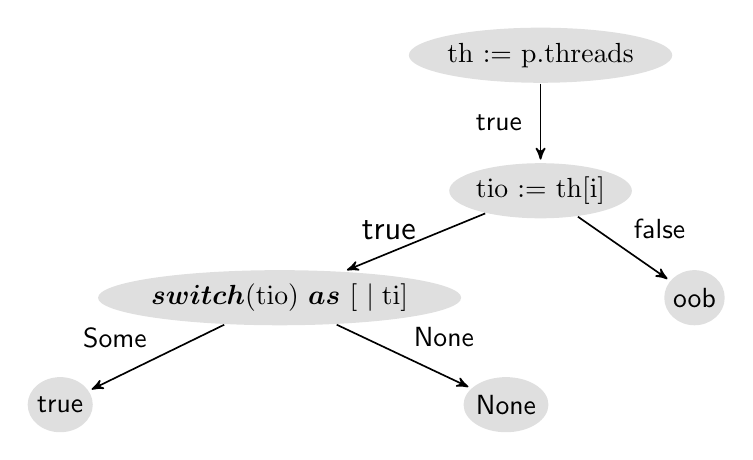
\begin{tikzpicture}[->,>=stealth',shorten >=1pt,auto,node distance=1.2cm, semithick,
    statt/.style={fill=lightgray!50,draw=none,text=black,ellipse,inner sep=0pt,minimum width=.7cm,minimum height=.7cm}]
%
   \node[statt]         (N1)  {{th := p.threads}};
   \node[statt]         (N2) [below=1cm of N1] { {tio := th[i]}};
   \node[statt]         (N3) [below left=of N2] { {$\boldsymbol{switch}$(tio) $\boldsymbol{as}$ 
                             [ $\ver$ti}]};
   \node[statt]         (N4) [below right=of N2]{\textsf{oob}};
   \node[statt]         (N5) [below left=of N3]{\lbtrue};
   \node[statt]         (N6) [below right=of N3]{\textsf{None}};  
   \path (N1) edge              node[xshift=-0.95cm] {{\lbtrue}} (N2);
   \path (N2) edge              node[xshift=-0.8cm,yshift = 0.4cm] {\large{\lbtrue}} (N3);
   \path (N2) edge              node {{\lbfalse}} (N4);
   \path (N3) edge              node[left, anchor=south east] { {\textsf{Some}}} (N5);
   \path (N3) edge              node[right, anchor=south west] { {\textsf{None}}} (N6);
\end{tikzpicture}
 }
\\
\bottomrule
\end{tabular}
}
\caption{$G_{\mathit{thread}}$ -- Control Flow Graph of Predicate \disp{thread}}
\label{pred:cfg:thread}
\end{figure}


\begin{figure}[hbtp]
\resizebox{0.95\textwidth}{!}{
\begin{tabular}{lll}
\toprule
\begin{tikzpicture}
\tikzset{
    position label/.style={
       below = 3pt,
       text height = 1.5ex,
       text depth = 1ex
    },
   brace/.style={
     decoration={brace},
     decorate
   }
}

\node at (3,9) {\Huge Exit label \lbtrue:};

\draw[dotted] (0,0) grid[xstep=8, ystep = 2] (8,8);
\fill[lightgray, opacity=0.2] (0,0) rectangle (8,8);
\node at (4,1) {\Huge adr\_space};
\node at (4,3) {\Huge crt\_thread};
\node at (4,5) {\Huge pid};
\node at (4,-1) {\Huge process p};
\draw[help lines] (0,6) grid[xstep=0.5, ystep = 2] (8,8);
\node at (1,7.5)  (nr) {} ;

\fill[caribbeangreen](2.5,6) rectangle (3,8);
\draw[pattern=north west lines, pattern color=black] (2.5,6) rectangle (3,8);
\node at (4,7) {\Huge threads};
\end{tikzpicture}
%
&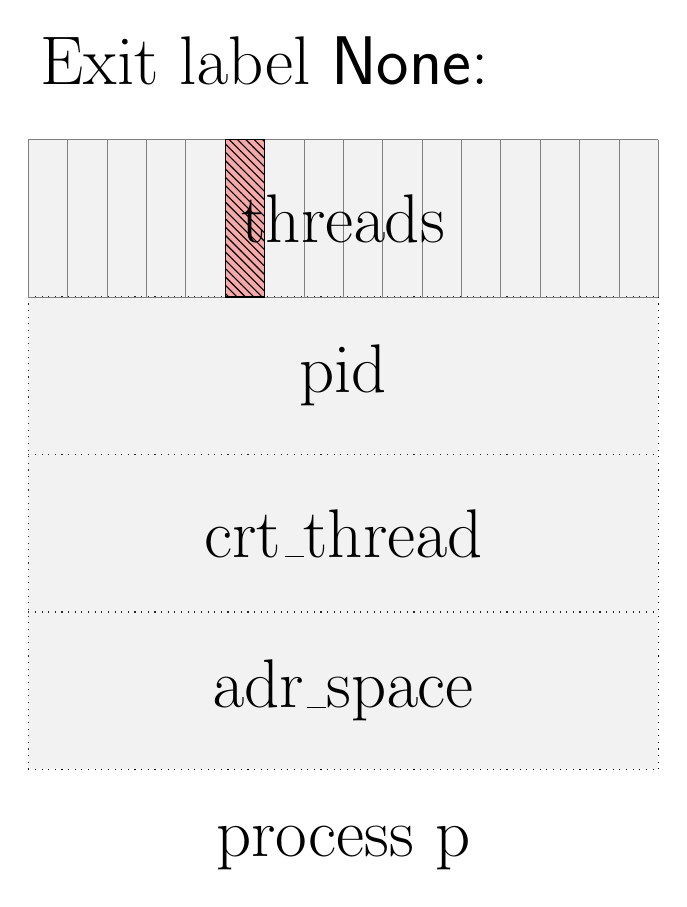
\begin{tikzpicture}
\tikzset{
    position label/.style={
       below = 3pt,
       text height = 1.5ex,
       text depth = 1ex
    },
   brace/.style={
     decoration={brace},
     decorate
   }
}
%
\node at (3,9) {\Huge Exit label \textsf{None}:};

\draw[dotted] (0,0) grid[xstep=8, ystep = 2] (8,8);
\fill[lightgray, opacity=0.2] (0,0) rectangle (8,8);
\node at (4,1) {\Huge adr\_space};
\node at (4,3) {\Huge crt\_thread};
\node at (4,5) {\Huge pid};
\node at (4,-1) {\Huge process p};
\draw[help lines] (0,6) grid[xstep=0.5, ystep = 2] (8,8);
\node at (1,7.5)  (nr) {} ;

\fill[red, opacity=0.3](2.5,6) rectangle (3,8);
\draw[pattern=north west lines, pattern color=black] (2.5,6) rectangle (3,8);
\node at (4,7) {\Huge threads};
\end{tikzpicture}
%
&\begin{tikzpicture}[node distance=0.5cm, legend-square/.style={draw=black!50!white, draw opacity=1, minimum width=1cm, minimum height=1cm, inner sep=0pt, anchor=north west}]
\node[anchor=base west] at (29,1.8) {\Large option<thread>:};
\node[fill=caribbeangreen,legend-square] (legend-green) at (29,1) {};
\node[right=of legend-green] {\Large Some(thread t)};
\node[fill=red,opacity=0.3,legend-square] (legend-red) at (29,-1) {};
\node[right=of legend-red]  {\Large None};

\node[pattern=north west lines, pattern color=black, preaction={fill=lightgray, opacity=0.2},legend-square] (legend-gray-lines) at (29,6) {};
\node[anchor=base west, right=of legend-gray-lines] {\Large Read/Needed};

\node[fill=lightgray, opacity=0.2, minimum width=1cm, minimum height=1cm,legend-square] (legend-gray) at (29,4) {};
\node[anchor=base west,right=of legend-gray] {\Large Irrelevant/Not Needed};

\path[draw=none,fill=none](29,-3.5) rectangle (31,0);
\end{tikzpicture}\\
\bottomrule
%
\end{tabular}
}
\caption{Targeted Dependency Results for Predicate \disp{thread}}
\label{ex:res:thread}
\end{figure}

Our dependency analysis should be able to distinguish between the different
exit labels of the predicate. For the label \disp{true} for instance, it
should detect that only the field \disp{threads} is read by the predicate,
while all others are irrelevant to the result. Furthermore, it should detect 
that for the \disp{threads} array of the input \disp{p} only the \disp{i}-th
element is inspected. Additionally, since we are considering the label 
\disp{true}, the \disp{i}-th element is necessarily an \emph{active} thread, 
indicated by the constructor \disp{Some}. The other constructor, \disp{None}, is 
\emph{impossible} for this execution scenario. On the contrary, for the exit 
label \disp{None}, the constructor \disp{Some} is impossible. For the exit label
\disp{oob}, nothing but the index \disp{i} and the ``support'' or ``length'' of the
associated \disp{threads} array is read. The targeted dependency results for the 
predicate \disp{thread} are depicted in Figure~\ref{ex:res:thread}.     
%% The second predicate, \disp{start_address}, whose control flow graph is shown in
%% Figure~\ref{ch4:pred:cfg:start}, receives a process \disp{p} and an index \disp{j} 
%% as inputs and finds the start address of the stack corresponding to an active thread. 

\begin{figure}[hbtp]\centering
\resizebox{0.7\textwidth}{!}{%
\begin{tabular}{@{}c@{}}
\toprule
{ \centering
  \hspace{1.6cm}
  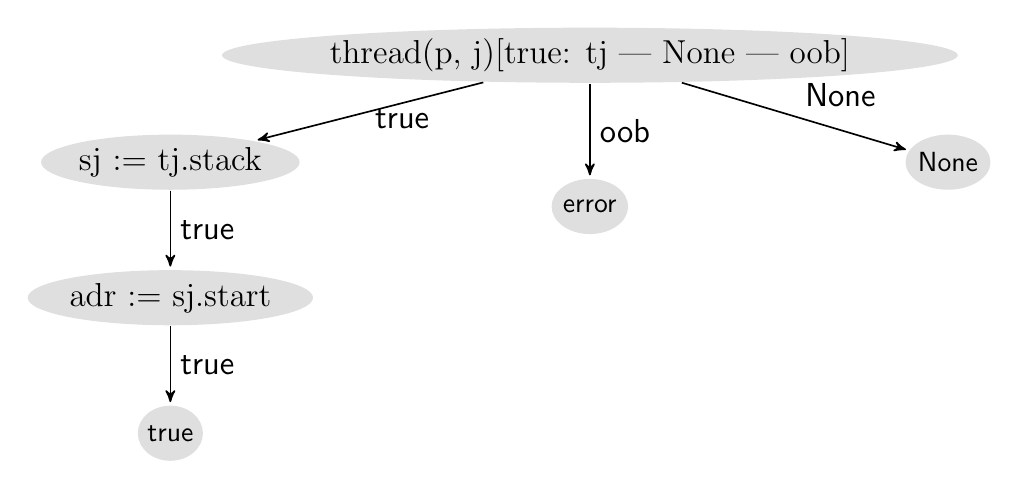
\begin{tikzpicture}[->,>=stealth',shorten >=1pt,auto,node distance=1.2cm, semithick,
    statt/.style={fill=lightgray!50,draw=none,text=black,ellipse,inner sep=0pt,minimum width=.7cm,minimum height=.7cm}]
%
   \node[statt]         (N1)  {\large {thread(p, j)[true: tj | None | oob]}};
   \node[statt]         (N2) [below left=of N1] {\large {sj := tj.stack}};
   \node[statt]         (N3) [below right=of N1] {\textsf{None}};
   \node[statt]         (N4) [below=1cm of N2]{\large {adr := sj.start}};
   \node[statt]         (N5) [below=1cm of N4]{\lbtrue}; 
   \node[statt]         (N6) [below=of N1]{\textsf{error}}; 
   \path (N1) edge              node[xshift=-0.05cm, yshift=0.15cm] {\large {\lbtrue}} (N2);
   \path (N1) edge              node {\large {\textsf{None}}} (N3); 
   \path (N2) edge              node {\large {\lbtrue}} (N4);
   \path (N4) edge              node{\large {\lbtrue}} (N5);
   \path (N1) edge              node {\large {\textsf{oob}}} (N6); 
\end{tikzpicture}
 }
\\
\bottomrule
\end{tabular}
}
\caption{$G_{\mathit{start\_address}}$ -- Control Flow Graph of Predicate \disp{start_address}}
\label{ch4:pred:cfg:start}
\end{figure}

The second predicate, \disp{start_address}, whose control flow graph is shown in
Figure~\ref{ch4:pred:cfg:start}, receives a process \disp{p} and an index \disp{j} 
as inputs and finds the start address of the stack corresponding to an active thread.
It makes a call to the predicate \disp{thread}, thus reading the 
\disp{j}-th element of the \disp{threads} array of its input process. If this is 
an active element, it further accesses the field \disp{stack}, from which it 
only reads the start address \disp{start}. Otherwise, if the element is inactive, 
the predicate forwards the exit label \disp{None} of the called predicate \disp{thread} 
and generates no output. When given an invalid index \disp{i}, the predicate exits
with label \disp{oob}. 
The predicate's implementation is shown in Figure~\ref{ex:start:code}.  

\begin{figure}[hbtp]
\begin{lstlisting}
predicate start_address(process p, int j)
 -> [true: int adr|None]
{{thread tj, memory_region sj}} {
  thread(p, j)[true: tj | None | oob] : [true -> 1, 
   None -> 4, oob -> 5];
  sj := tj.stack : [true -> 2];
  adr := sj.start : [true -> 3];
  [true];
  [None];
  [error] 
}
\end{lstlisting}
\caption{Predicate \disp{start_address} -- Implementation}
\label{ex:start:code}
\end{figure}

The dependency information for this predicate should capture the fact that on the
\disp{true} execution scenario, only the field \disp{start} of the input's 
\disp{j}-th associated thread is read. Furthermore, the only possible constructor
on this execution path is the \disp{Some} constructor. On the contrary, for the
\disp{None} execution scenario the only possible constructor is the \disp{None}
constructor. The targeted dependency results for the \disp{start_address} 
predicate are depicted in Figure~\ref{ex:res:start}. We remark that for the \disp{oob}
execution scenario, only the ``support'' or ``length'' of the \disp{threads} array is
read. 
  
\begin{figure}[hbtp]
\resizebox{0.95\textwidth}{!}{
\begin{tabular}{lll}
\toprule
\begin{tikzpicture}
\tikzset{
    position label/.style={
       below = 3pt,
       text height = 1.5ex,
       text depth = 1ex
    },
   brace/.style={
     decoration={brace},
     decorate
   }
}

\node at (3,9) {\Huge Exit label \lbtrue:};

\draw[dotted] (0,0) grid[xstep=8, ystep = 2] (8,8);
\fill[lightgray, opacity=0.2] (0,0) rectangle (8,8);
\node at (4,1) {\Huge adr\_space};
\node at (4,3) {\Huge crt\_thread};
\node at (4,5) {\Huge pid};
\node at (4,-1) {\Huge process p};
\draw[help lines] (0,6) grid[xstep=0.5, ystep = 2] (8,8);
\node at (1,7.5)  (nr) {} ;

\fill[caribbeangreen](2.5,6) rectangle (3,8);
\node (tj) at (2.8,7.8) {};
\node at (4,7) {\Huge threads};

\draw[dotted] (9,11) rectangle (12,12);
\fill[lightgray, opacity=0.2] (9,11) rectangle (12,12);
\node at (10.5,11.5) {\huge id};

\draw[dotted] (9,10) rectangle (12,11);
\fill[lightgray, opacity=0.2] (9,10) rectangle (12,11);
\node at (10.5,10.5) {\Large crt\_state};

\draw[dotted] (9,9) rectangle (12,10);
\fill[lightgray, opacity=0.2] (9,9) rectangle (12,10);
\node (s) at (10.5,9.5) {\Large stack};
\node (s2) at (9, 9.5) {};
\node at (10.5,8.5) {\huge thread tj};


\draw[dotted] (14,9) rectangle (16,10);
\fill[lightgray, opacity=0.2] (14,9) rectangle (16,10);
\draw[pattern=north west lines, pattern color=black, opacity=0.5] (14,9) rectangle (16,10);
\node (a) at (15,9.5) {\Huge start};
\node at (16,8.5) {\huge stack stj};

\draw[dotted] (16,9) rectangle (18,10);
\fill[lightgray, opacity=0.2] (16,9) rectangle (18,10);
\node at (17,9.5) {\huge length};

\draw[->, very thick] (s) edge (a); 
\draw[->, very thick, out=90] (tj) edge (s2);

\end{tikzpicture}
%
&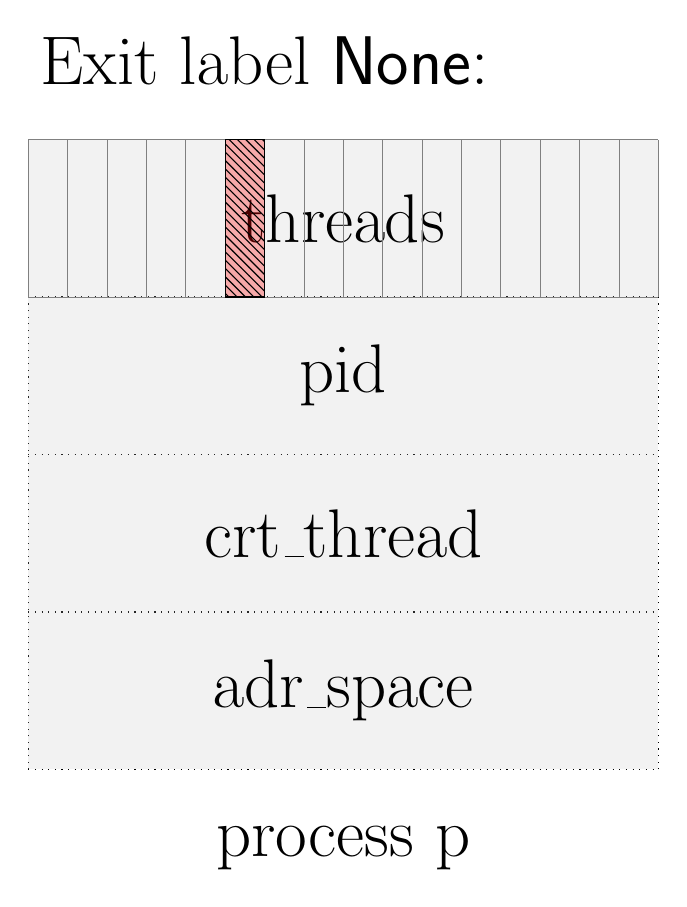
\begin{tikzpicture}
\tikzset{
    position label/.style={
       below = 3pt,
       text height = 1.5ex,
       text depth = 1ex
    },
   brace/.style={
     decoration={brace},
     decorate
   }
}
%
\node at (3,9) {\Huge Exit label \textsf{None}:};

\draw[dotted] (0,0) grid[xstep=8, ystep = 2] (8,8);
\fill[lightgray, opacity=0.2] (0,0) rectangle (8,8);
\node at (4,1) {\Huge adr\_space};
\node at (4,3) {\Huge crt\_thread};
\node at (4,5) {\Huge pid};
\node at (4,7) {\Huge threads};
\node at (4,-1) {\Huge process p};
\draw[help lines] (0,6) grid[xstep=0.5, ystep = 2] (8,8);
\node at (1,7.5)  (nr) {} ;

\fill[red, opacity=0.3](2.5,6) rectangle (3,8);
\draw[pattern=north west lines, pattern color=black] (2.5,6) rectangle (3,8);
%\draw[dotted, red] (2.5,6) rectangle (3,8);
\end{tikzpicture}
%
&\begin{tikzpicture}[node distance=0.5cm, legend-square/.style={draw=black!50!white, draw opacity=1, minimum width=1cm, minimum height=1cm, inner sep=0pt, anchor=north west}]
\node[anchor=base west] at (29,1.8) {\Large option<thread>:};
\node[fill=caribbeangreen,legend-square] (legend-green) at (29,1) {};
\node[right=of legend-green] {\Large Some(thread t)};
\node[fill=red,opacity=0.3,legend-square] (legend-red) at (29,-1) {};
\node[right=of legend-red]  {\Large None};

\node[pattern=north west lines, pattern color=black, preaction={fill=lightgray, opacity=0.2},legend-square] (legend-gray-lines) at (29,6) {};
\node[anchor=base west, right=of legend-gray-lines] {\Large Read/Needed};

\node[fill=lightgray, opacity=0.2, minimum width=1cm, minimum height=1cm,legend-square] (legend-gray) at (29,4) {};
\node[anchor=base west,right=of legend-gray] {\Large Irrelevant/Not Needed};

\path[draw=none,fill=none](29,-3.5) rectangle (31,0);
\end{tikzpicture}\\
\bottomrule
%
\end{tabular}
}
\caption{Targeted Dependency Results for Predicate \disp{start_address}}
\label{ex:res:start}
\end{figure}

\subsection{The dependency abstract domain}
\label{sec:depdom}

The first step towards inferring expressive, type-sensitive results that capture
the dependency specific to each subelement of an algebraic data type or an 
associative array, is the definition of an \emph{abstract dependency domain} 
%\defsymbol{$\udep$}{Abstract dependency domain}%
$\udep$, that mimics the structure of such data types. The dependency domain $\delta \in 
\udep$, shown below, is defined inductively from the three atomic cases --- 
$\everything$, $\nothing$ and $\impossible$ --- and mirrors the structure of the 
concrete types. 
%
\begin{definition}\label{ch5depdom}{Dependency Domain $\delta \in 
\udep$.}
\[
\begin{array}{lllr}
\dom := &\ver \everything &\textrm{\emph{Everything} -- atomic case} &\snumber{i}\\
        &\ver \nothing    &\textrm{\emph{Nothing} -- atomic case} &\snumber{ii}\\
        &\ver \impossible &\textrm{\emph{Impossible} -- atomic case} &\snumber{iii}\\
        &\ver \structdom{\dstruct{1}}{\dstruct{n}} &f_1, \ldots, f_n \textrm{ fields} &\snumber{iv}\\
        &\ver \vardom{\dvar{1}}{\dvar{m}} & C_1, \ldots, C_m  \textrm{ constructors}  &\snumber{v}\\
        &\ver \adom{\dom} & &\snumber{vi}                      \\
        &\ver \addef & i \; \textrm{array index} & \snumber{vii}\\
\end{array}
\]
\end{definition}
%
\noindent As reflected by the above definition, the dependency for atomic types
is expressed in terms of the domain's atomic cases: \everything{} (least
precise), denoting that \emph{everything} is needed and \nothing, denoting that
\emph{nothing} is needed. The third atomic case \impossible, denoting
\emph{impossible}, is introduced for the \emph{possible constructors} analysis
performed simultaneously, and is further explained below.

The dependency of a structure {\snumber{iv}} describes the dependency on each of 
its fields. %% For example, the dependency assigned to a structure having three 
%% fields, $f$, $g$ and $h$, in the context of a predicate operating on it and 
%% reading only the $h$ field, while ignoring the other two fields, could be of the 
%% following form: $\{f \mapsto \oslash, g \mapsto \oslash, h \mapsto \top \}$. 
For instance, revisiting our \disp{thread} example from 
Section~\ref{sec:intro:example}, we could express an over-approximation of the 
dependency information depicted for the process \disp{p} in 
Figure~\ref{ex:res:thread} using the following dependency: 
%
\[
\{\mathit{threads} \mapsto \top; \; \mathit{pid} \mapsto \oslash; \; 
\mathit{crt\_thread} \mapsto \oslash; \; \mathit{adr\_space} \mapsto \oslash \}.\]
%
This captures the fact that all fields except the \disp{threads} field are 
irrelevant, i.e. they are not read and \emph{nothing} in their contents is 
needed. The dependency for the \disp{threads} field is an over-approximation
and expresses the fact that it is entirely necessary, i.e. \emph{everything} in 
its value is needed for the result.   

For arrays we distinguish between two cases, namely arrays with a general 
dependency applying to all of the cells {given by \snumber{vi}} and arrays with a 
general dependency applying to \emph{all but one} exceptional cell, for which a specific 
dependency is known {given by \snumber{vii}}. %% For example, the dependency assigned to an
%% array having elements of the structured type with three fields used above, 
%% considered in the context of a predicate reading only the field $h$ of the $i$-th
%% array element and ignoring everything else, could be of the following form:
%% $\aexcdom{\oslash}{i}{\{f \mapsto \oslash, g \mapsto \oslash, h \mapsto \top \}}$.
For instance, for the \disp{threads} field of the previous example, the 
following dependency:
%
\[
\aexcdom{\oslash}{i}{\top}
\]
%
would be a less coarse approximation, capturing the fact that only the \disp{i}-th 
element of the associated \disp{threads} array is needed, while all others are 
irrelevant.

For variants {\snumber{v}}, the dependency is expressed in terms of the 
dependencies of their constructors, expressed in turn in terms of their 
arguments' dependencies. Thus, a constructor having a dependency mapped to 
\nothing{} is one for which nothing but the \emph{tag} has been read, i.e. its 
arguments, if any, are irrelevant for the execution. %% For instance, the dependency assigned to a 
%% variant having two constructors $A$ and $B$, in the context of a predicate that
%% only reads the tag for the $A$ constructor and depends completely on the $B$
%% constructor, could be of the following form:
%% $[A \mapsto \oslash; B \mapsto \top]$. 
For instance, for the \disp{i}-th element of the \disp{threads} array of our 
previous example, the following dependency:
%
\[
[\mathit{Some} \mapsto \top; \mathit{None} \mapsto \oslash]
\]
%
would be a more precise approximation, when considering the exit label 
\disp{true}. It is still an over-approximation as it expresses that both
constructors are possible. The argument of the \disp{Some} constructor is
entirely read, while for \disp{None} only the tag is read. 
%% This expresses the fact that the only possible constructor is 
%% \disp{Some} and that its argument is entirely read.

For variants, we want to take a step further and to also include the information 
that certain constructors cannot occur for certain execution paths. \emph{Impossible}, the third 
atomic case --- \impossible{} --- is introduced for this purpose. As mentioned 
previously in Section~\ref{sec:intro}, in order to obtain this additional 
information, we perform a ``possible-constructors'' analysis simultaneously, 
which computes for each execution scenario, the subset of possible constructors 
for a given value, at a given program point. All constructors that cannot occur 
on a given execution path are marked as being \impossible. In contrast, 
constructors for which \emph{only} the tag is read are marked as $\oslash$. The 
difference between $\impossible$ and $\nothing$ can be illustrated by 
considering a polymorphic option type \emph{option<A>}, having two constructors, 
$None$ and $\mathit{Some(A \, val)}$, respectively, and a Boolean predicate that 
pattern matches on an input of this type and returns \emph{false} in the case of 
$None$ and \emph{true} in the case of $Some$, unconditioned by the value $val$ of 
its argument. For the \emph{true} execution scenario, the dependency on the 
$Some$ constructor would be $\oslash$. The tag is read and it is decisive for the 
outcome, but the value of its argument $val$ is completely irrelevant. The 
dependency on the $None$ constructor however would be $\impossible$: the 
predicate can exit with label \emph{true} if and only if the input matches 
against the $Some$ constructor. By distinguishing between these two cases we 
can not only distinguish the input's subelements that have a direct impact on an 
operation's output, but additionally, we can also obtain a more detailed 
footprint that highlights the influence exerted by the input's ``shape'' on the 
operation's outcome.

For instance, for the \disp{i}-th element of the \disp{threads} array of our 
previous example, a dependency mapping the constructor \disp{None} to $\bot$
would be a more precise approximation, when considering the label \disp{true}.
Taking into account all the discussed values, we can express the dependency 
depicted in Figure~\ref{ex:res:thread} for the label \disp{true} as follows:

\[
\left \{
\begin{array}{lll}
\mathit{threads} &\mapsto & \aexcdom{\oslash}{i}{[\mathit{Some} \mapsto \top; \mathit{None} \mapsto \bot]}\\
\mathit{pid} &\mapsto &\oslash \\
\mathit{crt\_thread} &\mapsto &\oslash \\
\mathit{adr\_space} &\mapsto &\oslash\\
\end{array}
\right\}.
\]

We remark that $\top$, $\oslash$ and $\bot$ can apply to any type. For 
instance, $\top$ can be seen as a placeholder for data that is needed in its
entirety. Structure, array or variant dependencies whose subelements are all
entirely needed and thus, uniformly mapped to $\top$, are transformed to $\top$.
The $\bot$ dependency is a placeholder for data that cannot occur on a certain
execution scenario. A whole variant value is impossible if all its constructors
are mapped to $\bot$. A whole structure or array is impossible if any of its
subelements is impossible.
 
The {\impossible} atomic value is the lower bound of our domain and hence, the 
most precise value. The final abstract dependency is a closure of all these combined 
recursively. To give an intuition of the shape of our dependency lattice, we 
illustrate below in Figure~\ref{hasse} the Hasse diagram of the order relation 
between pairs of atomic dependency values. Intuitively, if the two analyses would
be performed separately, the upper ``diamond'' shape would correspond to the 
dependency analysis, and the lower one to the possible-constructors analysis. The
$\oslash$ element would be the lower bound for the dependency domain and the upper
bound for the possible-constructors domain. By performing them simultaneously, 
$\bot$ becomes the domain's lower bound.

\begin{center}
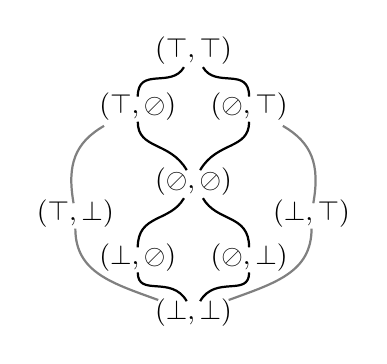
\begin{tikzpicture}
    \node (top) at (0,0) {$(\top,\top)$};
    \node [below left  of=top] (left)  {$(\top, \oslash)$};
    \node [below right of=top] (right) {$(\oslash, \top)$};
    \node [below right of=left,yshift=-0.25cm] (middle) {$(\oslash, \oslash)$};

    \node [below left of=middle, yshift=-0.25cm] (lowerleft)  {$(\bot, \oslash)$};
    \node [below right of=middle,yshift=-0.25cm] (lowerright) {$(\oslash, \bot)$};

    \node [below right of=lowerleft] (bot) {$(\bot, \bot)$};

    \node [above right of=lowerleft, xshift=-1.5cm, yshift=-4.25] (inbetleft)  {$(\top, \bot)$};
    \node [above left of=lowerright, xshift=1.5cm, yshift=-4.25] (inbetright) {$(\bot, \top)$};

    \draw [thick, shorten <=-3pt, shorten >=-5pt, out=-120, in=90] (top) to (left);
    \draw [thick, shorten <=-3pt, shorten >=-5pt, out=-60,  in=90] (top) to (right);

    \draw [thick, shorten <=-5pt, shorten >=-3pt, out=120, in=-90] (middle) to (left);
    \draw [thick, shorten <=-5pt, shorten >=-3pt, out=60,  in=-90] (middle) to (right);

    \draw [thick, shorten <=-3pt, shorten >=-5pt, out=-120, in=90] (middle) to (lowerleft);
    \draw [thick, shorten <=-3pt, shorten >=-5pt, out=-60,  in=90] (middle) to (lowerright);

    \draw [thick, shorten <=-5pt, shorten >=-3pt, out=120, in=-90] (bot) to (lowerleft);
    \draw [thick, shorten <=-5pt, shorten >=-3pt, out=60,  in=-90] (bot) to (lowerright);

    \draw [gray, thick, shorten <=-5pt, shorten >=-3pt, out=160, in=-90] (bot) to (inbetleft);
    \draw [gray, thick, shorten <=-5pt, shorten >=-3pt, out=20,  in=-90] (bot) to (inbetright);

    \draw [gray, thick, shorten <=-5pt, shorten >=-3pt, out=100, in=-150] (inbetleft) to (left);
    \draw [gray, thick, shorten <=-5pt, shorten >=-3pt, out=80,  in=-30] (inbetright) to (right);
\end{tikzpicture}
\captionof{figure}{Order Relation on Pairs of Atomic Dependencies}
\label{hasse}
\end{center}

\subsection{Dependency flow equations}
The intraprocedural dependency analysis keeps dependency information at each point 
of the control flow graph, for each  input, output and local
variables. 

\begin{definition}{Intraprocedural Dependency Domain $\intra \in \uintra$.}\label{ch5:intradom:definition}
The \emph{intraprocedural} dependency domain $\uintra$ is defined as 
%
\[\intra \ni \uintra =  \mathcal{V} \rightarrow \udep\]
% 
An element of this domain is a mapping from variables to dependencies.
\end{definition}


Our dependency analysis is a \emph{backward} data-flow analysis. For each exit 
label, it traverses the control flow graph starting with its corresponding exit 
node and it marks all other exit points as \emph{Unreachable}, since exit labels
are mutually exclusive. The intraprocedural domain for the currently analysed 
label is initialized with its associated output variables mapped to \everything. 
Thereby, the analysis starts by making a conservative approximation and by
considering that all the input has been observed and the output depends on it 
entirely. Typically, dependence analyses are \emph{forward} analyses. However, 
given our goal to express \emph{label-specific} dependencies as input-output 
relations and taking into consideration the characteristics of the {\asmil} 
language, choosing to design our analysis as a backward data-flow analysis 
seemed a pertinent choice. In {\asmil}, outputs are associated to a particular 
exit label and they are generated if and only if the predicate exits with that 
particular label. By traversing the control flow graph backwards, we can use
this information and consider, starting with the initialisation phase, only the outputs
that are relevant for the analysed exit label.  

After the initialisation, the analysis then traverses the control flow graph and
gradually refines the dependencies until a fixed point is reached.
Table~\ref{representation} summarizes the representation and general equation of
the statements. For each statement, the presented data-flow equation operates on
the intraprocedural domains of the statement's \emph{successor} nodes. The
intraprocedural domain at the \emph{entry point} of the node is obtained by
\emph{joining} the contributions of each \emph{outgoing} edge as shown in
Figure~\ref{intra:contrib:entry}.


\definecolor{indianred}{rgb}{0.90, 0.80, 0.71} %melon
\tikzstyle{vertex} = [ellipse, fill=lightgray!50, minimum size =30pt, inner sep = 0pt]
\tikzstyle{edge} = [draw, semithick, -> ] 
\begin{figure}[hbt]\centering
\begin{tabular}{@{}c@{}}
\toprule
\begin{tikzpicture}
[scale=0.4, auto]
\node[vertex] (n1) at (10.5,14) {\phantom{switch }\Large{\textsf{statement}}\phantom{switch}}; 
\draw[edge] (10.5,16.3) -- (10.5,15.2); 
\node [above](l1) at (6.5, 16.15) {$\Delta_{in} = \;$};
%% \node [above](l9) at (14.95, 16.1) {$ \;[(\Delta_{\lambda_1}\!\setminus \textrm{\textsf{gen}})\oplus \transfer{.}{s}{\lambda_1}]\vee \ldots \vee [(\Delta_{\lambda_n}\!\setminus \textrm{\textsf{gen}})\oplus \transfer{.}{s}
%% {\lambda_n}] \;$};
\node [above](l9) at (14.95, 16.1) {$ \; \transfer{\Delta_{\lambda_1}}{s}{\lambda_1} \ijoin \ldots \ijoin
\transfer{\Delta_{\lambda_n}}{s}{\lambda_n}\;$};
\node (contrib) at (23.2, 15.2) {\small $\transfer{\Delta_i}{s}{\lambda_i} : (\Delta_i \setminus 
\textrm{\textsf{gen}}_{s, \lambda_i}) \ireduce \delta_{s,\lambda_i}$} ;
\node (line2) at (24.2, 14) {\small $\delta_{s,\lambda_i}$ contribution of $s$ on $\lambda_i$};

\draw[edge] (8.5, 12.75) -- (7.5, 9.5);
\node [below](l2) at (6.5, 11.9) {\small $\delta_{s,\lambda_1}$};
\node [above](l3) at (6.6, 9.4) {$\Delta_{\lambda_{1}}$};
\draw[edge] (12.5, 12.75) -- (13.5, 9.5);
\node [below](l6) at (10.5, 12.5) {$\ldots$};
\node [below](l4) at (14.5, 11.9) {\small $\delta_{s,\lambda_n}$};
\node [above](l5) at (14.5, 9.4) {$\Delta_{\lambda_{n}}$};
\node [below](l7) at (4.1, 12.9) {\footnotesize ($\Delta_{\lambda_1}\!\setminus \textrm{\textsf{gen}}_{s,\lambda_1}$) $\ireduce \delta_{s,\lambda_1} $};
\node [below](l8) at (17, 12.9) {\footnotesize ($\Delta_{\lambda_n}\!\setminus \textrm{\textsf{gen}}_{s,\lambda_n}$) $\ireduce \delta_{s,\lambda_n}$};
\end{tikzpicture} \\
\bottomrule
\end{tabular}
\caption{Computation of the Intraprocedural Domain at a Node's Entry Point}
\label{intra:contrib:entry}
\end{figure}

Table~\ref{generic} presents the transfer functions for statements which are not 
type-specific. For equality tests \snumber{1} both of the inputs $e_1$, $e_2$ are 
completely read, whether the test returns \lbtrue{} or \lbfalse. The transfer 
functions therefore, reduce the domain of the corresponding successor node with
a domain consisting of $e_1$ and $e_2$ both mapped to $\everything$.
%
In the case of assignment \snumber{2}, the dependency of the written output 
variable $o$ is forgotten from the successor's intraprocedural domain, thus 
being mapped to \nothing{} and forwarded to the input variable $e$.
%
The transfer function for the $\unop$ operation \snumber{3} is simply the 
identity.

\begin{longtable}{@{}c@{}}
\caption{Generic Statements -- Data-Flow Equations}
\ra{1.4}
\label{generic}
\endlastfoot
\resizebox{0.99\linewidth}{!}{
$
\begin{array}{@{}lll@{}}
\toprule
\textsf{Statement} & & \transfer {\intra}{s}{\lambda_i}
\\
\midrule
%
%Equality test
\textrm{\textsf{Equality test}}  & (1)
%
&\begin{tabular}{@{}lcccl@{}}
 $ \transfer{\intra}{e_1 = e_2}{\textrm{\lbtrue}} = \displaystyle \intra \; \ireduce\;  dep $
&&&& where 
%
\\
$\transfer{\intra}{e_1 = e_2}{\textrm{\lbfalse}} = \displaystyle \intra \; \ireduce\;  dep
    $ 
&&&&  
$ dep = \left \{ 
\begin{array} {lcl}
           e_1 & \mapsto \top \\
           e_2 & \mapsto \top
           \end{array}

  \right \} $
\\
\end{tabular}
%
\\ \\
%
%Assignment
 \textrm{\textsf{Assignment}} & (2) 
%
&  \transfer{\intra}{o:=e}{\lbtrue} =  \displaystyle \killo{}{o} \; \ireduce \; 
   \{ e \mapsto \intra(o) \}\\\\
%Nop
\textrm{\textsf{No Operation}} & (3) &\transfer{\intra}{\unop}{\lbtrue} = \intra \\\\
\bottomrule
\end{array}
$ 
}
\end{longtable}
%

The data-flow equations given in Table~\ref{structures} correspond to 
structure-related statements. For the equations \snumber{4}, \snumber{5}, 
\snumber{6} and \snumber{7} we assume that the variable $r$ is of type 
$\commonstype$ for some fields $f_i,\; 1 \leq i \leq n$. The equation \snumber{4} 
refers to the creation of a structure: each input $e_i$ is read as much as the 
corresponding field $f_i$ of the structure is read.
%
The destructuring of a structure is handled in \snumber{5}: each field $f_i$ is 
needed as much as the corresponding variable $o_i$ is.
%
When accessing the $i$-th field of a structure $r$ \snumber{6}, only the field 
$f_i$ is read, and only as much as the access' result $o$ itself. 
% 
The equation \snumber{7} treats field updates: the variable $e_i$ is read as much 
as the field $f_i$ is. The structure $r$ is read as much as all the fields other 
than $f_i$ are read in $r'$.  
%
Finally, the equations given in \snumber{8} handle partial structure equality 
tests, and the transfer functions are the same for the labels \lbtrue{} or 
\lbfalse: for both compared structures $r'$ and $r''$, all the fields in the given 
set $f_1, \ldots, f_k$ are completely read, and only those.

\begin{longtable}{@{}c@{}}
\caption{Structure-Related Statements -- Data-Flow Equations}
\ra{1.3}
\label{structures}
\endlastfoot
\resizebox{0.99\linewidth}{!}{
$
\begin{array}{@{}lcl@{}}
\toprule
 \textsf{Statement} & &  \transfer {\intra}{s}{\lambda_i} \\ 
\midrule 
%Create Structure
\textrm{\textsf{Create}} & \textrm{(4)}
&  \transfer{\intra}{\recordnew}{\textrm{\textsf{\lbtrue}}} = 
\displaystyle \killo {}{r} \; \ireduce \; \displaystyle \bigoplus_{1\leq i \leq n}\{e_i \mapsto \intra(r).f_i \}\\\\ 
% Destruct structure
\textrm{\textsf{Destructure}} & \textrm{(5)}   
& \transfer{\intra}{\recordall}{\textrm{\textsf{\lbtrue}}} =  
\displaystyle \killo {}{ \{o_i \ver o_i \in \bar{o} \}} \; \ireduce \; 
\displaystyle \{r \mapsto \{f_1 \mapsto\intra(o_1); \ldots; f_n \mapsto \intra(o_n)\}\}\\\\
% Field Access
\textrm{\textsf{Access field}} & \textrm{(6)}
&  \transfer{\intra}{\recordget}{\textrm{\textsf{\lbtrue}}} = 
\displaystyle \killo {}{o} \; \ireduce \; \{r \mapsto \{f_1 \mapsto \oslash; \ldots;  
 f_i \mapsto \intra(o); \ldots; f_n \mapsto \oslash \} \}\\\\
% Field Update
\textrm{\textsf{Update field}} & \textrm{(7)}   
&  \transfer{\intra}{\recordset}{\textrm{\textsf{\lbtrue}}} =
       \displaystyle \killo{}{r'}
             \; \ireduce \;
             \left \{
             \begin{array}{lll}
             e_i & \mapsto & \intra(r').f_i \\ 
             r & \mapsto & \left \{ \displaystyle
             f_1 \mapsto \delta_1; \ldots ; f_n \mapsto \delta_n
             \right \} 
             \end{array}
             \right \} \\\\
&& \textrm{where }             \delta_j = \left \{
                \begin{array}{ll}
                \intra(r').f_j & \textrm{if $j \neq i $} \\
                \oslash & \textrm{otherwise}\\
                \end{array} \right . \\\\
% Structure Equality
\textrm{\textsf{Equality}} & \textrm{(8)}   
& 
\begin{tabular}{@{}lccl@{}}
$\transfer{\intra}{\recordeq}{\lbtrue} = \displaystyle 
 \intra \; \ireduce \; d$  
&&& 
%\textrm{where}
$ \textrm{where } d =   \left \{
  \begin{array} {lll}
  r' & \mapsto & \displaystyle \left \{ f_1 \mapsto \delta_1; \ldots ; f_n \mapsto \delta_n  
  \right \} \\
  r'' & \mapsto & \displaystyle \left \{ f_1 \mapsto \delta_1; \ldots; f_n \mapsto \delta_n      
 \right  \}
  \end{array}
  \right \}
\;
  $ \\\\
$\transfer{\intra}{\recordeq}{\lbfalse} = \displaystyle 
 \intra \; \ireduce \; d $
&&& $\textrm{and } \delta_i =   \left \{
  \begin{array} {ll}
  \top & \textrm{if } f_i \in \{f_1, \ldots, f_k\}\\
  \oslash & \textrm{otherwise} 
  \end{array}
  \right.
\;
  $ 
\end{tabular}\\ \\
\bottomrule
\end{array}
$
}
\end{longtable}


%%% More tables for arrays and variants at line 1985 in Chapter5.tex


\subsection{Intraprocedural Dependency Analysis Illustrated}\label{sec:intra:example}

To better illustrate our analysis at an intraprocedural level, we exemplify
the mechanism behind it, step by step, on the predicate \disp{thread}, discussed
in Section~\ref{sec:intro:example}. We consider the \disp{true} execution 
scenario, apply our dependency analysis and compare the actual obtained results 
with the targeted ones depicted in Figure~\ref{ex:res:thread}.

\definecolor{indianred}{rgb}{0.90, 0.80, 0.71} %melon
\definecolor{burg}{rgb}{0.8, 0.36, 0.36}
\tikzstyle{vertex} = [ellipse, fill=lightgray!50, minimum size =30pt, inner sep = 0pt]
\tikzstyle{lvertex} = [circle, fill=lightgray!50, minimum size=30pt, inner sep=0pt]
\tikzstyle{ivertex} = [circle, draw=red, minimum size=30pt, inner sep = 0pt]
\tikzstyle{edge} = [draw, semithick, -> ] 
\tikzstyle{edgeRed} = [draw=red!50!black, dashed, thick, -> ] 
\begin{figure}[h]\centering
\begin{tabular}{@{}c@{}}
\toprule
%% \begin{tikzpicture}
%% [scale=0.6, auto]
%% \node[vertex] (n1) at (10,14) {\emph{threads := p.threads}}; 
%% \node[vertex] (n2) at (10,11) {\emph{tio := threads[i]}};
%% \node[vertex] (n3) at (10,8) {\emph{switch(tio) as [ti$\arrowvert\;$]}}; 

%% \node (n4) [draw=red!50!black, circle,fill=lightgray!50, minimum size=30pt, inner sep =0pt] at(8,5.5) {\emph{true}};
%% \draw[draw=red!50!black] (8,5.5) circle(20pt); 

%% \node (n5) [draw=red!50!black, circle,fill=lightgray!50, minimum size=30pt, inner sep =0pt] at(12,5.5) {\emph{None}}; 
%% \draw[draw=red!50!black] (12,5.5) circle(20pt); 

%%   \foreach \from/\to in {n1/n2,n2/n3,n3/n4,n3/n5}{
%%     \draw[edge] (\from) -- (\to); 
%%   }

%%   \draw (n2.-30) edge[semithick,->,bend left,in=120] (n5.30); 

%% \node(n8) [draw=indianred!50, fill = indianred!50, scale=0.7] at (17.5, 4) {
%% \textrm{thread(p, i) $\to$ [true: ti $\ver$ None]}}; 

%% \node(n9)[draw=burg, scale = 0.8] at (15.75,5.5) {
%% \begin{tabular}{c}
%%  $ \mathit{Unreachable} $\\
%% \end{tabular}
%% };

%% \node(d1) [draw=caribbeangreen, scale = 0.9] at (3,5.5) {
%% \begin{tabular}{c}
%% ti $\mapsto$ $\top$\\
%% \end{tabular}
%% }; 

%% \end{tikzpicture}
  \begin{tikzpicture}[->,>=stealth',shorten >=1pt,auto,node distance=1.2cm, semithick,
    statt/.style={scale=0.7,fill=lightgray!50,draw=none,text=black,ellipse,inner sep=0pt,minimum width=.7cm,minimum height=.7cm}]
%
   \node[statt]         (N1)  {\large {th := p.threads}};
   \node[statt]         (N2) [below=1cm of N1] {\large {tio := th[i]}};
   \node[statt]         (N3) [below left=of N2] {\large {$\boldsymbol{switch}$(tio) $\boldsymbol{as}$ 
                             [ $\ver$ti}]};
   \node[statt]         (N4) [below right=of N2]{\textsf{oob}};
   \node[statt]         (N5) [below left=of N3]{\lbtrue};
   \node[statt]         (N6) [below right=of N3]{\textsf{None}};  
   \path (N1) edge              node[xshift=-0.95cm] {\large {\lbtrue}} (N2);
   \path (N2) edge              node[xshift=-0.8cm,yshift = 0.4cm] {\large{\lbtrue}} (N3);
   \path (N2) edge              node {\large {\lbfalse}} (N4);
   \path (N3) edge              node[left, anchor=south east] {\large {\textsf{Some}}} (N5);
   \path (N3) edge              node[right, anchor=south west] {\large {\textsf{None}}} (N6);

\node(n8)[draw=burg,dotted, scale = 0.7, right=of N4, xshift=-1.6cm] {
\begin{tabular}{c}
 $ \mathit{Unreachable} $\\
\end{tabular}
};

\node(n9)[draw=burg,dotted, scale = 0.7, right=of N6] {
\begin{tabular}{c}
 $ \mathit{Unreachable} $\\
\end{tabular}
};

\node(d1) [draw=caribbeangreen, scale = 0.9, left=of N5] {
\begin{tabular}{c}
ti $\mapsto$ $\top$\\
\end{tabular}
}; 
\end{tikzpicture}\\
\bottomrule
\end{tabular}
\caption{Analysing Predicate \disp{thread} -- Initialisation}
\label{intra:ss:init}
\end{figure}
 
Since a predicate can only exit with one label at a time and we are considering 
the \disp{true} label, we can map the nodes \disp{None} and \disp{oob} to 
\emph{Unreachable}, as shown in Figure~\ref{intra:ss:init}. This is an advantage
of backwards analyses. For \disp{true}, we 
make a pessimistic assumption and map the output \disp{ti} to {\everything}, 
considering that control on the output is external and hence, out of our reach,
and that \disp{ti} will be entirely needed by a potential caller. Going further 
up the control flow graph, we analyse the \emph{variant switch}.

In order to compute the dependency for the node corresponding to the variant 
switch, we apply the data-flow equation, given by \snumber{10} in 
Table~\ref{variants}. Since we are analysing the \disp{true} case, we know that 
all other constructors (only the constructor \disp{None} in this case) are 
locally impossible. Thus, we map it to $\bot$. We continue by forgetting the 
dependency information we knew about the output \disp{ti}. Since its value is 
needed only in as much as the result of the switch on the corresponding edge is 
needed, we forward it to the part corresponding to the \disp{Some} constructor.
This is summarized below:

\begin{figure}[!h]\centering
\begin{tabular}{c}
%\begin{table}{@{}c@{}}
\toprule
    \begin{tikzpicture}[
      dot/.style={circle,inner sep=0pt,minimum size=1mm,fill=black},
      ]
      
      \matrix[inner sep=0pt,ampersand replacement=\&] (mtop) {
        \dottriangle{(0,0)}{1}{}{5}{4}{};\&
        \node[resetinnersep, anchor=base,yshift=-.2cm] (dots2) {$\vphantom{x}\dots\vphantom{x}$};\& 
        \coordinate (myorigin);
           \dottriangle{(0,0)}{ia}{}{5}{4}{};
        \coordinate[xshift=.15cm] (coord-ib) at (dottriangle-isep-ia.east |- myorigin);
          \node[anchor=west,inner sep=0pt] (ioplus) at (dottriangle-boundingbox-ia.east) {$\vphantom{x}\mathbin{\oplus}\vphantom{x}\;$};
          \dottriangle{(ioplus.east |- myorigin)}{ib}{green!50!black}{5}{4}{fill=green!50!black!30!white};
         {
          \node[anchor=west,inner sep=0pt,opacity=0] (ioplus) at (dottriangle-boundingbox-ia.east) {$\vphantom{x}\mathbin{\oplus}\vphantom{x}\;$};
          \dottriangle{(ioplus.east |- myorigin)}{ib}{green!50!black,opacity=0}{5}{4}{fill=green!50!black!30!white,opacity=0};
        }
        \&
        \node[resetinnersep, anchor=base,yshift=-.2cm] (dotsn1) {$\vphantom{x}\dots\vphantom{x}$};\& 
        \dottriangle{(0,0)}{n}{}{5}{4}{}; \\
      };

      % Draw bottoms on top:
        \node[fit=(dottriangle-bg-1),fill=red!20!white,inner sep=0pt,opacity=.9]  {};
        \node[green!50!black] at (dottriangle-bg-1.center) {$\bot$};
        \node[fit=(dottriangle-bg-n),fill=red!20!white,inner sep=0pt,opacity=.9]  {};
        \node[green!50!black] at (dottriangle-bg-n.center) {$\bot$};

      \draw (dottriangle-isep-1.east |- mtop.north) -- (dottriangle-isep-1.east |- mtop.south);
      \draw (dots2.east |- mtop.north) -- (dots2.east |- mtop.south);
      \draw (dottriangle-isep-ib.east |- mtop.north) -- (dottriangle-isep-ib.east |- mtop.south);
      \draw (dotsn1.east |- mtop.north) -- (dotsn1.east |- mtop.south);

      \node[resetinnersep,anchor=south,yshift=.3cm] at (dottriangle-dot-1 |- mtop.north) (num1) {\footnotesize$C_1$};
      \path ($(dottriangle-dot-ia)!.5!(dottriangle-dot-ib)$) |- node[resetinnersep,anchor=south,yshift=.3cm] (numi) {\footnotesize$C_{Some}$} (mtop.north);
      \node[resetinnersep,anchor=south,yshift=.3cm] at (dottriangle-dot-n |- mtop.north) (numn) {\footnotesize$C_n$};

      \node[inner sep=0pt,fit=(num1) (numi) (numn)] (mnum) {};
      \node[inner sep=0pt,fit=(mtop) (mnum)] (mall) {};
      
      \path[fill=black!7] (mnum.south west -| mall.west) -- (mnum.south east -| mall.east) -- (mtop.north east -| mall.east) -- (mtop.north west -| mall.west) -- cycle;
      \path (mnum.south west -| mall.west) edge[draw] (mnum.south east -| mall.east) -- (mtop.north east -| mall.east) edge[draw] (mtop.north west -| mall.west) -- cycle;
      \draw (mall.north west) -- (mall.north east) -- (mall.south east) -- (mall.south west) -- cycle;
      
      \node[anchor=base east,xshift=\defaultinnersep] (a) at (dottriangle-x-1.base -| mall.west) {$\mathit{tio} =\vphantom{x}$};
      
      \node[below left,yshift=-3mm] (o) at (mall.south west) {$\mathit{ti} =$};
      
        \dottriangle{(o.base east)}{o}{red}{5}{4}{fill=red!30!white};
        % cross out:
        \node[draw=red,cross out,inner sep=0pt,minimum width=.75cm,minimum height=.55cm,thick,opacity=.5] at (dottriangle-bg-o) {}; 
      {
        \dottriangle{(o.base east)}{o}{}{5}{4}{};
      }

        \draw (dottriangle-tc-o) edge[->,>=stealth,bend right,thick,green!30!black] (dottriangle-tc-ib);
      ;
    \end{tikzpicture}\\
  %\end{figure}

 \definecolor{indianred}{rgb}{0.8, 0.36, 0.36}

$
\colorbox{lightgray!50}{
\begin{tabular}{@{}l@{}}
$\transfer{\intra}{\varswitch}{\lambda_i} = 
\displaystyle (\intra \setminus o_i) \oplus \{ v \mapsto dep_i\}$ 
\\
where \\ 
$dep_i = [\colorbox{indianred}{$C_1 \mapsto \bot;$} \ldots; \colorbox{green!50!black!30!white}{$C_i \mapsto \intra(o_i);$} \ldots; \colorbox{indianred}{$C_n \mapsto \bot$}]$
\end{tabular}}
%\bottomrule
$ \\
\bottomrule
\end{tabular}
\caption{Applying the Variant Switch Equation}
\end{figure}

\definecolor{indianred}{rgb}{0.8, 0.36, 0.36}

\begin{figure}[h]\centering
\begin{tabular}{c}
\toprule
\resizebox{0.99\textwidth}{!}{%
%% \begin{tikzpicture}
%% [scale=0.6, auto]
%% \node[vertex] (n1) at (10,14) {\emph{threads := p.threads}}; 
%% \node[vertex] (n2) at (10,11) {\emph{tio := threads[i]}};
%% \node[vertex] (n3) at (10,8) {\emph{switch(tio) as [ti$\arrowvert\;$]}}; 

%% \node (n4) [draw=red!50!black, circle,fill=lightgray!50, minimum size=30pt, inner sep =0pt] at(8,5.5) {\emph{true}};
%% \draw[draw=red!50!black] (8,5.5) circle(20pt); 

%% \node (n5) [draw=red!50!black, circle,fill=lightgray!50, minimum size=30pt, inner sep =0pt] at(12,5.5) {\emph{None}}; 
%% \draw[draw=red!50!black] (12,5.5) circle(20pt); 

%%   \foreach \from/\to in {n1/n2,n2/n3,n3/n4,n3/n5}{
%%     \draw[edge] (\from) -- (\to); 
%%   }

%%   \draw (n2.-30) edge[semithick,->,bend left,in=120] (n5.30); 

%% \node(n8) [draw=indianred!50, fill = indianred!50, scale=0.7] at (17.5, 4) {
%% \textrm{thread(p, i) $\to$ [true: ti $\ver$ None]}}; 

%% \node(n9)[draw=burg, scale = 0.8] at (15.75,5.5) {
%% \begin{tabular}{c}
%%  $ \mathit{Unreachable} $\\
%% \end{tabular}
%% };

%% \node(d2) [draw=caribbeangreen, scale=0.8] at (2.5,8) {
%% \begin{tabular}{ccc}
%% tio & $\mapsto$ & [Some $\mapsto \top$; None $\mapsto \bot$]  \\
%% \end{tabular}
%% };

%% \node(d1) [draw=caribbeangreen, scale = 0.9] at (3,5.5) {
%% \begin{tabular}{c}
%% ti $\mapsto$ $\top$\\
%% \end{tabular}
%% }; 

%% \end{tikzpicture}
  \begin{tikzpicture}[->,>=stealth',shorten >=1pt,auto,node distance=1.2cm, semithick,
    statt/.style={scale=0.7,fill=lightgray!50,draw=none,text=black,ellipse,inner sep=0pt,minimum width=.7cm,minimum height=.7cm}]
%
   \node[statt]         (N1)  {\large {th := p.threads}};
   \node[statt]         (N2) [below=1cm of N1] {\large {tio := th[i]}};
   \node[statt]         (N3) [below left=of N2] {\large {$\boldsymbol{switch}$(tio) $\boldsymbol{as}$ 
                             [ $\ver$ti}]};
   \node[statt]         (N4) [below right=of N2]{\textsf{oob}};
   \node[statt]         (N5) [below left=of N3]{\lbtrue};
   \node[statt]         (N6) [below right=of N3]{\textsf{None}};  
   \path (N1) edge              node[xshift=-0.95cm] {\large {\lbtrue}} (N2);
   \path (N2) edge              node[xshift=-0.8cm,yshift = 0.4cm] {\large{\lbtrue}} (N3);
   \path (N2) edge              node {\large {\lbfalse}} (N4);
   \path (N3) edge              node[left, anchor=south east] {\large {\textsf{Some}}} (N5);
   \path (N3) edge              node[right, anchor=south west] {\large {\textsf{None}}} (N6);

\node(n8)[draw=burg,dotted, scale = 0.7, right=of N4, xshift=-1.6cm] {
\begin{tabular}{c}
 $ \mathit{Unreachable} $\\
\end{tabular}
};

\node(n9)[draw=burg,dotted, scale = 0.7, right=of N6] {
\begin{tabular}{c}
 $ \mathit{Unreachable} $\\
\end{tabular}
};

\node(d2) [draw=caribbeangreen, scale=0.8, left=of N3]  {
\begin{tabular}{ccc}
tio & $\mapsto$ & [Some $\mapsto \top$; None $\mapsto \bot$]  \\
\end{tabular}
};

\node(d1) [draw=caribbeangreen, scale = 0.9, left=of N5] {
\begin{tabular}{c}
ti $\mapsto$ $\top$\\
\end{tabular}
}; 
\end{tikzpicture}
}\\
\bottomrule
\end{tabular}
\caption{Analysing Predicate \disp{thread} -- Variant Switch}
\label{intra:ss:switch}
\end{figure}

Taking all this into account, for the node corresponding to the variant switch, 
we obtain the dependency shown in Figure~\ref{intra:ss:switch}. For the output 
\disp{ti}, we depend entirely on the \disp{Some} constructor of the node's 
input variant \disp{tio}, while the constructor \disp{None} is impossible.

Making a step further up the graph, we access the cell \disp{i} of the array 
\disp{th} and apply the equation \snumber{12} given in Table~\ref{arrays}. 
We begin by forgetting the dependency for the output \disp{tio}, 
since this is written. Since we only access the element \disp{i}, we map all 
other cells to \emph{Nothing}, i.e. $\oslash$. To the dependency corresponding 
to the \disp{i}-th cell, we forward the dependency we knew about \disp{tio}, 
since we depend on it to the extent to which the result of the access is needed.

\begin{figure}[!h]\centering
\begin{tabular}{c}
\toprule
        \begin{tikzpicture}[
      dot/.style={circle,inner sep=0pt,minimum size=1mm,fill=black},
      ]
      
      \matrix[inner sep=0pt,ampersand replacement=\&] (mtop) {
        \dottriangle{(0,0)}{1}{}{5}{4}{};
          \node[anchor=west,inner sep=1.3mm,xshift=-1.3mm] (1oplus) at (dottriangle-boundingbox-1.east) 
            {$\vphantom{x}\mathbin{\oplus}\textcolor{green!50!black}{\oslash}$};
        {
          \node[anchor=west,inner sep=1.3mm,xshift=-1.3mm,opacity=0] (1oplus) at (dottriangle-boundingbox-1.east) 
{$\vphantom{x}\mathbin{\oplus}\textcolor{green!50!black}{\oslash}$};
        } \&
        \node[resetinnersep, anchor=base,yshift=-.2cm] (dots2) {$\vphantom{x}\dots\vphantom{x}$};\& 
        \coordinate (myorigin);
        \dottriangle{(0,0)}{ia}{}{5}{4}{};
        %\alt<3->{
          \node[anchor=west,inner sep=0pt] (ioplus) at (dottriangle-boundingbox-ia.east) 
            {$\vphantom{x}\mathbin{\oplus}\vphantom{x}\;$};
          \dottriangle{(ioplus.east |- myorigin)}{ib}{green!50!black}{5}{4}{fill=green!50!black!30!white};
        {
          \node[anchor=west,inner sep=0pt,opacity=0] (ioplus) at (dottriangle-boundingbox-ia.east) 
{$\vphantom{x}\mathbin{\oplus}\vphantom{x}\;$};
          \dottriangle{(ioplus.east |- myorigin)}{ib}{green!50!black,opacity=0}{5}{4}{fill=green!50!black!30!white,opacity=0};
        }\&
        \node[resetinnersep, anchor=base,yshift=-.2cm] (dotsn1) {$\vphantom{x}\dots\vphantom{x}$};\& 
        % \dottriangle{(0,0)}{n1}{}{5}{4}{}; \&
        \dottriangle{(0,0)}{n}{}{5}{4}{};
       
          \node[anchor=west,inner sep=1.3mm,xshift=-1.3mm] (noplus) at (dottriangle-boundingbox-n.east) 
            {$\vphantom{x}\mathbin{\oplus}\textcolor{green!50!black}{\oslash}$};
        {
          \node[anchor=west,inner sep=1.3mm,xshift=-1.3mm,opacity=0] (noplus) at (dottriangle-boundingbox-n.east) 
{$\vphantom{x}\mathbin{\oplus}\textcolor{green!50!black}{\oslash}$};
        } \\
      };
      
      \draw (1oplus.east |- mtop.north) -- (1oplus.east |- mtop.south);
      \draw (dots2.east |- mtop.north) -- (dots2.east |- mtop.south);
      \draw (dottriangle-isep-ib.east |- mtop.north) -- (dottriangle-isep-ib.east |- mtop.south);
      \draw (dotsn1.east |- mtop.north) -- (dotsn1.east |- mtop.south);

      \node[resetinnersep,anchor=south] at (dottriangle-dot-1 |- mtop.north) (num1) {\footnotesize$1$};
      \path ($(dottriangle-dot-ia)!.5!(dottriangle-dot-ib)$) |- node[resetinnersep,anchor=south] (numi) {\footnotesize$i$} (mtop.north);
      \node[resetinnersep,anchor=south] at (dottriangle-dot-n |- mtop.north) (numn) {\footnotesize$n$};

      \node[inner sep=0pt,fit=(num1) (numi) (numn)] (mnum) {};
      \node[inner sep=0pt,fit=(mtop) (mnum),draw] (mall) {};
      
      \draw (mtop.north west) -- (mtop.north east);
      
      \node[anchor=base east,xshift=\defaultinnersep] (a) at (dottriangle-x-1.base -| mall.west) {$\mathit{th} =\vphantom{x}$};
      
      \node[below left,yshift=-3mm] (o) at (mall.south west) {$\mathit{tio} =$};
      
        \dottriangle{(o.base east)}{o}{red}{5}{4}{fill=red!30!white};
        % cross out:
        \node[draw=red,cross out,inner sep=0pt,minimum width=.75cm,minimum height=.55cm,thick,opacity=.5] at (dottriangle-bg-o) {};
      {
        \dottriangle{(o.base east)}{o}{}{5}{4}{};
      }

% {
          \node[draw=red,cross out,inner sep=0pt,minimum width=.75cm,minimum height=.55cm,thick,opacity=0] at (dottriangle-bg-ia) {};

        \draw (dottriangle-tc-o) edge[->,>=stealth,bend right,thick,green!30!black] (dottriangle-tc-ib);
      ;
    \end{tikzpicture}\\


\resizebox{0.95\textwidth}{!}{
\colorbox{lightgray!50}{
$\transfer{\intra}{\arrayget}{\lbtrue} = \displaystyle
 \left \lgroup
               \begin {array}{ll}
                \colorbox{indianred}{$\killo{}{o} $}\; \oplus \;
                \left \{
                \begin{array}{lll}
                i & \mapsto & \top \\%{green!50!black!30!white}
                a & \mapsto & \colorbox{green!50!black!30!white}{$\langle \oslash \; \triangleright \; i: \intra(o) \rangle$}
                \end{array} \right \} 
               & \begin{array}{l}
                 \textrm{when $ i \in \inputs \;$} \\                
                 \end{array}
       \\ \\
                \colorbox{indianred}{$\killo{}{o}$} \; \oplus \; 
                \left \{
                \begin{array} {lll}
                 i & \mapsto & \top \\
                 a & \mapsto &\colorbox{green!50!black!30!white}{$ \langle \intra(o) \vee \oslash \rangle$}
                 \end{array}
                \right \} 
               & \begin{array}{l}
                 \textrm {when $ i \notin \inputs \;$} \\                 
                 \end{array}
              \\
               \end{array} \right.
 $
}}\\
\bottomrule
\end{tabular}
\caption{Applying the Array Access Equation}
\label{fig:eq:array}
\end{figure}

We thus obtain a dependency stating that we depend only on the \disp{i}-th 
cell of the array \disp{th}, for which only the constructor \disp{Some} is 
possible and entirely needed. The cell's index \disp{i} is entirely needed as 
well. The applied equation is shown in Figure~\ref{fig:eq:array} (since \disp{i}
is an input, we use the first case of the equation) and the 
obtained results are shown in Figure~\ref{intra:ss:array}. 

\begin{figure}[h]\centering
\begin{tabular}{@{}c@{}}
\toprule
\resizebox{0.99\textwidth}{!}{%
%% \begin{tikzpicture}
%% [scale=0.6, auto]
%% \node[vertex] (n1) at (10,14) {\emph{threads := p.threads}}; 
%% \node[vertex] (n2) at (10,11) {\emph{tio := threads[i]}};
%% \node[vertex] (n3) at (10,8) {\emph{switch(tio) as [ti$\arrowvert\;$]}}; 

%% \node (n4) [draw=red!50!black, circle,fill=lightgray!50, minimum size=30pt, inner sep =0pt] at(8,5.5) {\emph{true}};
%% \draw[draw=red!50!black] (8,5.5) circle(20pt); 

%% \node (n5) [draw=red!50!black, circle,fill=lightgray!50, minimum size=30pt, inner sep =0pt] at(12,5.5) {\emph{None}}; 
%% \draw[draw=red!50!black] (12,5.5) circle(20pt); 

%%   \foreach \from/\to in {n1/n2,n2/n3,n3/n4,n3/n5}{
%%     \draw[edge] (\from) -- (\to); 
%%   }

%%   \draw (n2.-30) edge[semithick,->,bend left,in=120] (n5.30); 

%% \node(n8) [draw=indianred!50, fill = indianred!50, scale=0.7] at (17.5, 4) {
%% \textrm{thread(p, i) $\to$ [true: ti $\ver$ None]}}; 

%% \node(n9)[draw=burg, scale = 0.8] at (15.75,5.5) {
%% \begin{tabular}{c}
%%  $ \mathit{Unreachable} $\\
%% \end{tabular}
%% };

%% \node(d3) [draw=caribbeangreen, scale=0.8] at (1.4,10.8) {
%% \begin{tabular}{cll}
%% threads & $\mapsto $
%% & $\langle \oslash\;\; \triangleright\;$  i: [Some $\mapsto \top$; None $\mapsto \bot$] $\rangle$  \\

%% i & $\mapsto$ &$\top$\\
%% \end{tabular}
%% };

%% \node(d2) [draw=caribbeangreen, scale=0.8] at (2.5,8) {
%% \begin{tabular}{ccc}
%% tio & $\mapsto$ & [Some $\mapsto \top$; None $\mapsto \bot$]  \\
%% \end{tabular}
%% };

%% \node(d1) [draw=caribbeangreen, scale = 0.9] at (3,5.5) {
%% \begin{tabular}{c}
%% ti $\mapsto$ $\top$\\
%% \end{tabular}
%% }; 

%% \end{tikzpicture}
 \begin{tikzpicture}[->,>=stealth',shorten >=1pt,auto,node distance=1.2cm, semithick,
    statt/.style={scale=0.7,fill=lightgray!50,draw=none,text=black,ellipse,inner sep=0pt,minimum width=.7cm,minimum height=.7cm}]
%
   \node[statt]         (N1)  {\large {th := p.threads}};
   \node[statt]         (N2) [below=1cm of N1] {\large {tio := th[i]}};
   \node[statt]         (N3) [below left=of N2] {\large {$\boldsymbol{switch}$(tio) $\boldsymbol{as}$ 
                             [ $\ver$ti}]};
   \node[statt]         (N4) [below right=of N2]{\textsf{oob}};
   \node[statt]         (N5) [below left=of N3]{\lbtrue};
   \node[statt]         (N6) [below right=of N3]{\textsf{None}};  
   \path (N1) edge              node[xshift=-0.95cm] {\large {\lbtrue}} (N2);
   \path (N2) edge              node[xshift=-0.8cm,yshift = 0.4cm] {\large{\lbtrue}} (N3);
   \path (N2) edge              node {\large {\lbfalse}} (N4);
   \path (N3) edge              node[left, anchor=south east] {\large {\textsf{Some}}} (N5);
   \path (N3) edge              node[right, anchor=south west] {\large {\textsf{None}}} (N6);

\node(n8)[draw=burg,dotted, scale = 0.7, right=of N4, xshift=-1.6cm] {
\begin{tabular}{c}
 $ \mathit{Unreachable} $\\
\end{tabular}
};

\node(n9)[draw=burg,dotted, scale = 0.7, right=of N6] {
\begin{tabular}{c}
 $ \mathit{Unreachable} $\\
\end{tabular}
};

\node(d3) [draw=caribbeangreen, scale=0.8, left=of N2] {
\begin{tabular}{cll}
th & $\mapsto $
& $\langle \oslash\;\; \triangleright\;$  i: [Some $\mapsto \top$; None $\mapsto \bot$] $\rangle$  \\
i & $\mapsto$ &$\top$\\
\end{tabular}
};

\node(d2) [draw=caribbeangreen, scale=0.8, left=of N3]  {
\begin{tabular}{ccc}
tio & $\mapsto$ & [Some $\mapsto \top$; None $\mapsto \bot$]  \\
\end{tabular}
};

\node(d1) [draw=caribbeangreen, scale = 0.9, left=of N5] {
\begin{tabular}{c}
ti $\mapsto$ $\top$\\
\end{tabular}
}; 
\end{tikzpicture}
}\\
\bottomrule
\end{tabular}
\caption{Analysing Predicate \disp{thread} -- Array Access}
\label{intra:ss:array}
\end{figure}

As a last step, we access the field \disp{threads} of the input process \disp{p}
and apply the equation \snumber{6} given in Table~\ref{structures} and illustrated in
Figure~\ref{intra:ss:faccess}.
As before, we forget the information for \disp{th}, the access result. We 
map all other fields to $\oslash$ and we forward the dependency of the variable 
\disp{th} to the dependency part of the field \disp{threads}.

\begin{figure}[!h]
\begin{tabular}{c}
\toprule
   % \centering   
    \begin{tikzpicture}[
      dot/.style={circle,inner sep=0pt,minimum size=1mm,fill=black},
%      every node/.style={draw=black!50!white}
      ]
      
      \matrix[inner sep=0pt,ampersand replacement=\&] (mtop) {
        \node[resetinnersep,] (f1) {$f_1=$}; \dottriangle{(f1.base east)}{1}{}{3}{4}{};
        %\alt<3->{
          \node[anchor=west,inner sep=1.3mm,xshift=-1.3mm] (1oplus) at (dottriangle-boundingbox-1.east)
          {$\vphantom{x}\mathbin{\oplus}\textcolor{green!50!black}{\oslash}$};
        {
          \node[anchor=west,inner sep=1.3mm,xshift=-1.3mm,opacity=0] (1oplus) at (dottriangle-boundingbox-1.east)
          {$\vphantom{x}\mathbin{\oplus}\textcolor{green!50!black}{\oslash}$};
        } \&
        \&
        \node[resetinnersep,] (f2) {$f_2=$}; \dottriangle{(f2.base east)}{2}{}{5}{4}{};
        %\alt<3->{
          \node[anchor=west,inner sep=1.3mm,xshift=-1.3mm] (2oplus) at (dottriangle-boundingbox-2.east)
          {$\vphantom{x}\mathbin{\oplus}\textcolor{green!50!black}{\oslash}$};
        {
          \node[anchor=west,inner sep=1.3mm,xshift=-1.3mm,opacity=0] (2oplus) at (dottriangle-boundingbox-2.east)
          {$\vphantom{x}\mathbin{\oplus}\textcolor{green!50!black}{\oslash}$};
        } \\
      };
      
      \matrix[inner sep=0pt,below=0cm of mtop, ampersand replacement=\&] (mmid) {
        \node[resetinnersep,] (fi) {$f_{threads}=\vphantom{x}$};
        % \alt<2->{
        % \dottriangle{([xshift=-\defaultinnersep]fi.base east)}{ia}{}{5}{3}{fill=red!30!white};
        % }{
        \dottriangle{([xshift=-\defaultinnersep]fi.base east)}{ia}{}{3}{5}{};
        % }
          \node[anchor=base west,inner sep=0pt] (ioplus) at (dottriangle-boundingbox-ia.east |- fi.base) {$\vphantom{x}\mathbin{\oplus}\vphantom{x}\;$};
          \dottriangle{(ioplus.base east)}{ib}{green!50!black}{3}{5}{fill=green!50!black!30!white};
        {
          \node[anchor=base west,inner sep=0pt,opacity=0] (ioplus) at (dottriangle-boundingbox-ia.east |- fi.base) {$\vphantom{x}\mathbin{\oplus}\vphantom{x}\;$};
          \dottriangle{(ioplus.base east)}{ib}{green!50!black,opacity=0}{3}{5}{fill=green!50!black!30!white,opacity=0};
        }\\
      };

      \matrix[inner sep=0pt,below=0cm of mmid,ampersand replacement=\&] (mbot) {
        \node[resetinnersep,] (fn1) {$f_{n-1}=$}; \dottriangle{(fn1.base east)}{n1}{}{4}{3}{};
          \node[anchor=west,inner sep=1.3mm,xshift=-1.3mm] (n1oplus) at (dottriangle-boundingbox-n1.east)
          {$\vphantom{x}\mathbin{\oplus}\textcolor{green!50!black}{\oslash}$};
        {
          \node[anchor=west,inner sep=1.3mm,xshift=-1.3mm,opacity=0] (n1oplus) at (dottriangle-boundingbox-n1.east)
          {$\vphantom{x}\mathbin{\oplus}\textcolor{green!50!black}{\oslash}$};
        } \&
        \node[resetinnersep,] (fn) {$f_{n}=$}; \dottriangle{(fn.base east)}{n}{}{4}{5}{};
        %\alt<3->{
          \node[anchor=west,inner sep=1.3mm,xshift=-1.3mm] (noplus) at (dottriangle-boundingbox-n.east)
          {$\vphantom{x}\mathbin{\oplus}\textcolor{green!50!black}{\oslash}$};
        {
          \node[anchor=west,inner sep=1.3mm,xshift=-1.3mm,opacity=0] (noplus) at (dottriangle-boundingbox-n.east)
          {$\vphantom{x}\mathbin{\oplus}\textcolor{green!50!black}{\oslash}$};
        } \\
      };
      
      \node[inner sep=0pt,fit=(mtop) (mmid) (mbot),draw] (mall) {};
      \draw (mtop.south -| mall.west) -- (mtop.south -| mall.east);
      \draw (mmid.south -| mall.west) -- (mmid.south -| mall.east);
      % \draw (f2.west |- mtop.north) -- (f2.west |- mtop.south);
      \draw (1oplus.east |- mtop.north) -- (1oplus.east |- mtop.south);
      % \draw (fn.west |- mbot.north) -- (fn.west |- mbot.south);
      \draw (n1oplus.east |- mbot.north) -- (n1oplus.east |- mbot.south);

      \node[anchor=base east,xshift=\defaultinnersep] (s) at (f1.base -| mall.west) {$p =\vphantom{x}$};
      
      \node[below left,yshift=-3mm] (o) at (mall.south west) {$th =$};
      
     
        \dottriangle{(o.base east)}{o}{red}{3}{5}{fill=red!30!white};
        % cross out:
        \node[draw=red,cross out,inner sep=0pt,minimum size=.55cm,thick,opacity=.5] at (dottriangle-bg-o) {};
      {
        \dottriangle{(o.base east)}{o}{}{3}{5}{};
      }

        \draw (dottriangle-tc-o) edge[->,>=stealth,bend right,thick,green!30!black] (dottriangle-tc-ib);
      
    \end{tikzpicture}\\

\colorbox{lightgray!50}{
$\transfer{\intra}{\recordget}{\textrm{\textsf{\lbtrue}}} = 
\displaystyle 
\colorbox{indianred} {$\killo {}{o}$} 
\; \oplus \; \{s \mapsto \{f_1 \mapsto \oslash; \ldots;  
\colorbox{green!50!black!30!white} {$f_i \mapsto \intra(o);$} 
\ldots; f_n \mapsto \oslash \} \} 
$
}\\
\bottomrule
\end{tabular}
\caption{Applying the Field Access Equation}
\label{intra:ss:faccess}
\end{figure} 

We thus obtain the dependency result shown in Figure~\ref{intra:ss:struct}. 
This states that for the label \disp{true}, the output \disp{ti} depends only on 
the \disp{i}-th cell of the field \disp{threads} of the input process \disp{p}, 
for which it depends entirely on the \disp{Some} constructor. Before returning
the predicate's final results, the analysis filters out any dependency 
information referring to local variables and verifies that the invariant imposed 
on dependency information related to arrays holds. Since the results refer only
to the inputs \disp{p} and \disp{i} and the index of the exceptional computed
dependency is an input, the invariant holds and the final result can be retrieved.
The final dependency results obtained for the \disp{thread} predicate on the exit
label \disp{true} are identical to the ones that we were targeting and that were
depicted in Figure~\ref{ex:res:thread}. For readability considerations, for 
structures such as the input process \disp{p}, we omit dependencies on fields
mapped to $\oslash$. We maintain this convention throughout the rest of this 
chapter, and thus any field of a structure that is omitted from a dependency
summary should be interpreted as being mapped to $\oslash$, i.e. \emph{nothing}.  

%de sters
%pana aici

\begin{figure}[htbp]\centering
\begin{tabular}{c}
\toprule
\resizebox{0.99\textwidth}{!}{%
%% \begin{tikzpicture}
%% [scale=0.6, auto]
%% \node[vertex] (n1) at (10,14) {\emph{threads := p.threads}}; 
%% \node[vertex] (n2) at (10,11) {\emph{tio := threads[i]}};
%% \node[vertex] (n3) at (10,8) {\emph{switch(tio) as [ti$\arrowvert\;$]}}; 

%% \node (n4) [draw=red!50!black, circle,fill=lightgray!50, minimum size=30pt, inner sep =0pt] at(8,5.5) {\emph{true}};
%% \draw[draw=red!50!black] (8,5.5) circle(20pt); 

%% \node (n5) [draw=red!50!black, circle,fill=lightgray!50, minimum size=30pt, inner sep =0pt] at(12,5.5) {\emph{None}}; 
%% \draw[draw=red!50!black] (12,5.5) circle(20pt); 

%%   \foreach \from/\to in {n1/n2,n2/n3,n3/n4,n3/n5}{
%%     \draw[edge] (\from) -- (\to); 
%%   }

%%   \draw (n2.-30) edge[semithick,->,bend left,in=120] (n5.30); 

%% \node(n8) [draw=indianred!50, fill = indianred!50, scale=0.7] at (17.5, 4) {
%% \textrm{thread(p, i) $\to$ [true: ti $\ver$ None]}}; 

%% \node(n9)[draw=burg, scale = 0.8] at (15.75,5.5) {
%% \begin{tabular}{c}
%%  $ \mathit{Unreachable} $\\
%% \end{tabular}
%% };

%% \node(d4) [draw=caribbeangreen, scale=0.7] at (0.6, 14) {
%% \begin{tabular}{lll}
%% p & $\mapsto $
%% & \{ threads $\mapsto$ $\langle \oslash\;\; \triangleright\; $ i:   
%% [Some $\mapsto \top$; \textrm{None $\mapsto \bot$}]$\rangle\}$ \\
%% i & $\mapsto$ & $\top$ \\
%% \end{tabular}
%% };

%% \node(d3) [draw=caribbeangreen, scale=0.8] at (1.4,10.8) {
%% \begin{tabular}{cll}
%% threads & $\mapsto $
%% & $\langle \oslash\;\; \triangleright\;$  i: [Some $\mapsto \top$; None $\mapsto \bot$] $\rangle$  \\

%% i & $\mapsto$ &$\top$\\
%% \end{tabular}
%% };

%% \node(d2) [draw=caribbeangreen, scale=0.8] at (2.5,8) {
%% \begin{tabular}{ccc}
%% tio & $\mapsto$ & [Some $\mapsto \top$; None $\mapsto \bot$]  \\
%% \end{tabular}
%% };

%% \node(d1) [draw=caribbeangreen, scale = 0.9] at (3,5.5) {
%% \begin{tabular}{c}
%% ti $\mapsto$ $\top$\\
%% \end{tabular}
%% }; 

%% \end{tikzpicture}

 \begin{tikzpicture}[->,>=stealth',shorten >=1pt,auto,node distance=1.2cm, semithick,
    statt/.style={scale=0.7,fill=lightgray!50,draw=none,text=black,ellipse,inner sep=0pt,minimum width=.7cm,minimum height=.7cm}]
%
   \node[statt]         (N1)  {\large {th := p.threads}};
   \node[statt]         (N2) [below=1cm of N1] {\large {tio := th[i]}};
   \node[statt]         (N3) [below left=of N2] {\large {$\boldsymbol{switch}$(tio) $\boldsymbol{as}$ 
                             [ $\ver$ti}]};
   \node[statt]         (N4) [below right=of N2]{\textsf{oob}};
   \node[statt]         (N5) [below left=of N3]{\lbtrue};
   \node[statt]         (N6) [below right=of N3]{\textsf{None}};  
   \path (N1) edge              node[xshift=-0.95cm] {\large {\lbtrue}} (N2);
   \path (N2) edge              node[xshift=-0.8cm,yshift = 0.4cm] {\large{\lbtrue}} (N3);
   \path (N2) edge              node {\large {\lbfalse}} (N4);
   \path (N3) edge              node[left, anchor=south east] {\large {\textsf{Some}}} (N5);
   \path (N3) edge              node[right, anchor=south west] {\large {\textsf{None}}} (N6);

\node(n8)[draw=burg,dotted, scale = 0.7, right=of N4, xshift=-1.6cm] {
\begin{tabular}{c}
 $ \mathit{Unreachable} $\\
\end{tabular}
};

\node(n9)[draw=burg,dotted, scale = 0.7, right=of N6] {
\begin{tabular}{c}
 $ \mathit{Unreachable} $\\
\end{tabular}
};

\node(d4) [draw=caribbeangreen, scale=0.7, left=of N1] {
\begin{tabular}{lll}
p & $\mapsto $
& \{ threads $\mapsto$ $\langle \oslash\;\; \triangleright\; $ i:   
[Some $\mapsto \top$; \textrm{None $\mapsto \bot$}]$\rangle\}$ \\
i & $\mapsto$ & $\top$ \\
\end{tabular}
};

\node(d3) [draw=caribbeangreen, scale=0.8, left=of N2] {
\begin{tabular}{cll}
th & $\mapsto $
& $\langle \oslash\;\; \triangleright\;$  i: [Some $\mapsto \top$; None $\mapsto \bot$] $\rangle$  \\

i & $\mapsto$ &$\top$\\
\end{tabular}
};

\node(d2) [draw=caribbeangreen, scale=0.8, left=of N3]  {
\begin{tabular}{ccc}
tio & $\mapsto$ & [Some $\mapsto \top$; None $\mapsto \bot$]  \\
\end{tabular}
};

\node(d1) [draw=caribbeangreen, scale = 0.9, left=of N5] {
\begin{tabular}{c}
ti $\mapsto$ $\top$\\
\end{tabular}
}; 
\end{tikzpicture}
}\\
\bottomrule
\end{tabular}
\caption{Analysing Predicate \disp{thread} -- Field Access}
\label{intra:ss:struct}
\end{figure}


\subsection{An inter-procedural extension}

\section{Correlation analysis}

\subsection{Introductory example}

\subsection{Correlations as partial equivalence relations}

\subsection{Correlation analysis}

\section{Experimental evaluation}

\section{Related work}

\section{Conclusions}

\bibliographystyle{alpha}
\bibliography{biblio}

\end{document}
